%% =====================================================================
%% BioMed-QAgent 参赛作品报告 — 主入口
%%
%% 本文件只保留:文档类、项目元信息、正文装配。
%% 所有排版(页面/字体/标题/页眉页脚/表格/代码/提示框)见:
%%   biomed-report.cls          — 模板入口
%%   biomed-report-theme.sty    — 视觉主题
%%
%% 编译(latexmk,产物在 build/):
%%   latexmk -xelatex -outdir=build main.tex
%% =====================================================================

\documentclass{biomed-report}

% ------------------------- 项目元信息 -------------------------
\reporttitle{BioMed QAgent}
\reportsubtitle{面向生物医学研究的多源数据智能采集与分析系统}
\reportshorttitle{BioMed QAgent · 参赛作品报告}
\reportschool{北京航空航天大学}
\reporttrack{赛道二-方向1A}
\reportdate{2026 年 9 月}

% ------------------------- 正文装配 -------------------------
\begin{document}

% 封面(不显示页码)
\makereporttitle

% 前置部分:目录(罗马页码)
\frontmatter

\tableofcontents

% 正文:从 1 开始的阿拉伯页码
\mainmatter

\chapter{引言}\label{ch:introduction}

\section{科研数据整理的真实困境}

生物医学研究中，“找到数据”不等于找到能用的数据。可以直接分析的数据集至少要说明：覆盖哪些实体和样本，来自哪个版本，原始文件如何转换为当前字段，不同来源能否合并，哪些值存在冲突，哪些判断需要研究者确认。只依靠对话和临时文件，难以逐项核对这些问题。

第一，同类数据也可能无法直接合并。相同列名未必代表相同测量；探针级与基因级表达表具有不同观测单位，原始强度、归一化值与对数值不能混用。生物活性数据还需对齐化合物标识、实验类型和单位，并记录冲突。

第二，可读信息不等于可计算数据。PDF 表格、扫描图、折线图与补充 XLSX 需要不同解析方法。视觉模型读取结果需附上页码、位置、模型名、提示版本与置信度，才能进一步复核。

第三，复制整理容易遗漏处理记录。在浏览器、Excel、脚本与聊天窗口之间反复搬运数据，可能丢失来源版本、筛选条件、字段映射与冲突处理依据，出现错误时难以回查。

第四，长任务需要保存运行状态。下载、权限审批和故障恢复可能跨越多个会话；仅依靠对话上下文，重启后容易重复操作或遗忘约束。

第五，来源分散且访问方式不同。同一问题可能涉及 PubMed、GEO、ClinVar、PDB 与论文附件。检索结果相关，不代表已经遍历分页、检查补充材料或覆盖全部必要来源。

\section{相关工作的实际缺口}\label{sec:related}

现有工作分别提供了检索、解析、数据整合和智能体编排能力。本文关注的是：这些环节产生的数据进入正式交付前，是否留下可逐项核对的来源、处理记录和发布检查结果。

数据库与解析工具解决查找和读取问题。PubMed、GEO、GDC、UniProt、ClinVar、ChEMBL 等提供专门查询入口；规则解析器适合固定格式，光学字符识别（Optical Character Recognition，OCR）与视觉语言模型（Vision-Language Model，VLM）用于读取页面和图像。跨库查询和字段对应仍需按任务设计。

数据整合与溯源工具提供了组织处理步骤和记录来源的方法。抽取—转换—加载（Extract–Transform–Load，ETL）流程适合执行明确的数据转换；W3C PROV、FAIR 和 OpenLineage 则提供来源描述或数据管理原则。应用仍需决定何时检查、如何拒绝不合格结果，以及怎样保留修正前后的文件。

LLM 编排与工作流框架可以支持工具调用、状态保存和人工介入，例如 LangGraph、AutoGen、OpenAI Agents SDK 与 Temporal\cite{langgraph,autogen,openai-agents,temporal-approval}。DocETL 提供查询改写与任务相关评估，Palimpzest 则在时长、费用和输出质量之间选择执行计划\cite{docetl,palimpzest}。这些能力可以用于构建发布检查，但框架支持某种检查，并不等于具体应用已经实现和验证了完整的数据交付流程。

本文将这些能力用于科研数据交付：来源登记后生成候选，候选经过检查与必要审批后正式发布，读取时再次核验。“信任边界”在本文中特指这条发布检查通道，不表示系统能自动证明科学内容正确。

\section{本系统的核心目标}

\mbox{BioMed QAgent} 聚焦于数据获取与处理，不替研究者作出科学结论。系统将自然语言需求转换为带有表结构、来源和检查记录的数据表，供后续分析使用，并支持根据反馈修正。

系统依次完成四项工作：

\begin{enumerate}
  \item 找得到：根据研究目标查找论文、数据库、附件、表格或图像。以 EGFR 突变体抑制实验为例，Agent 需要定位相关数据库和补充材料，并记录检索范围，而不只是返回相关网页。需求编译与来源发现见\ref{sec:requirement-compile} 节和\ref{sec:source-discovery} 节。
  \item 读得懂：将不同载体解析为字段含义明确的数据记录。例如表达表必须说明一行代表探针还是基因，不能仅凭列名推断。解析与规范化过程见第四章。
  \item 合得上：对齐实体标识和可换算的单位，同时保留缺失、重复和冲突。同一化合物的不同数据库标识需要映射，nM 与 $\mu$M 等单位差异需要按明确规则换算。
  \item 查得清：记录来源、输入摘要、处理版本、检查结果和人工修正。无法确认的内容应排除、标注或交研究者判断；正式发布与原始需求是否全部满足分别检查。
\end{enumerate}

上述流程对应来源发现、异构解析、清洗整合、图表提取与来源追溯。科研分析和结论生成不计入方向1A的正式交付要求。

\section{研究问题与数据需求}

本项目研究如何将自然语言数据需求转换为结构明确、处理步骤可检查的数据表。数据获取与整合属于本系统任务，后续假设验证与科学结论不属于正式交付范围。

用户输入自由文本后，系统从中确定数据集的十项选择，包括需要哪些数据、一行代表什么、从哪里采集、如何处理冲突等（表~\ref{tab:spec-choices}）。这些选择组成机器可读的数据集执行规格。规格确定了本次构建范围，但仍须与原始需求逐项核对，不能仅因规格执行成功就认为任务全部完成。

\begin{table}[htbp]
\centering
\caption{数据集规格的十项关键选择}\label{tab:spec-choices}
\begin{tabularx}{\linewidth}{>{\hsize=0.60000\hsize}L>{\hsize=1.20000\hsize}L>{\hsize=1.20000\hsize}L}
\toprule
\textbf{选择} & \textbf{含义} & \textbf{改变意味着什么} \\
\midrule
数据产品类别 & 本次需要哪一类数据产品 & 决定交付物的整体形态 \\
行层级 & 每行代表什么观测或统计单位 & 决定哪些行可合并、哪些需拆表 \\
目标表结构 & 交付表包含哪些字段及关系 & 决定字段映射、类型与检查规则 \\
实体集合 & 涉及哪些对象、范围多大 & 决定采集与筛选范围 \\
队列与筛选条件 & 按什么标准纳入或排除样本 & 改变样本总体与可比性 \\
来源与采集绑定 & 从哪个数据库或文件获取数据 & 决定可核对的来源 \\
规范化配置 & 采用哪些转换规则及参数 & 决定值的含义能否保持一致 \\
合并策略 & 重叠或冲突信息如何取舍 & 决定保留结果与冲突记录 \\
验证配置 & 采用哪些规则与阈值 & 决定发布检查标准 \\
输出格式 & 以什么格式交付 & 决定下游读取方式 \\
\bottomrule
\end{tabularx}
\end{table}

规格、来源文件、处理代码和参数均固定后，才有条件检查重复执行是否产生相同结果。重新发起来源检索或模型抽取，仍可能得到不同输入；样例1在 flash 与 max 下纳入研究不同，就是这种差异。第五章的哈希重验检查既有文件是否与清单一致，并非独立重跑实验。

相应地，系统交付的也不是一张孤立的数据表。合格的候选结果必须同时包含六类信息：数据本身、表结构、溯源信息、审计记录、验证结果、文件清单。候选结果只有通过全部质量检查后，系统才会生成正式发布版。正式发布只新增版本、不覆盖既有发布；读取时，系统依据发布清单重新校验文件摘要，发现文件缺失、损坏或与清单记录不一致即拒绝展示。

\section{主要贡献与核心机制}\label{sec:contributions}

本文提出三项相互配合的系统贡献，共同使用 Dataset Core 的八阶段流程。内容摘要、事件日志、模式检查和人工审批均为既有方法；本文将它们组合到同一次科研数据任务中，使候选文件在交付前接受统一检查。

\textbf{以可核验文件判定正式发布。}系统不将模型自报、工具预览或工作区 CSV 视为正式结果。Agent 提交规格，Core 完成处理与检查后生成发布清单。运行时向 Agent 提供真实进度，使其区分“仍在执行”“未能发布”和“已有正式发布物”。发布状态说明文件是否通过配置的检查；需求完成情况另按原始任务核对。

\textbf{检查运行时提出的表结构。}Agent 可以为未注册的多表任务提出表、字段、主外键与变换方案。候选文件必须说明输入来源，实际产生输出，并保证输出列与声明逐一对应。Core 重新计算文件摘要，再执行完整性检查、产品评估和发布检查；变换方不能自行选择或跳过这些模块。此处检查结构与来源是否一致，不自动判断变换计算是否正确。

\textbf{让人工确认对应具体证据。}审批请求携带任务身份、候选值与证据摘要。系统恢复操作前检查响应是否仍对应原请求和原对象；对象已变化或请求失效时，旧响应不能继续用于该对象。对已发起且要求人工处理的发布验收，只有人工接受后才继续发布。修正形成新版本，旧版文件与审批记录继续保留。各发布路径是否实际触发验收，须结合第五章运行记录判断。

来源文件、处理记录与发布清单共同说明数据从何而来、经过哪些步骤、最终交付哪些文件。摘要重验可以发现文件与记录不符，但摘要一致不等于数值正确，也不证明已经查全来源。这两项仍需对照原始来源和任务要求核验。


\chapter{问题定义}\label{ch:problem-definition}

\section{任务边界}

本系统支持的核心任务是：给定医学研究对象和数据需求，发现并采集一个或多个科学数据来源，将其转换为统一的单表或多表结构，保留来源和处理记录，并输出便于后续分析的CSV 数据产品。

相应地，本系统不把下列事项作为正式交付承诺：自动提出并验证科学假设，替代领域专家判断数据的科学含义，对研究结果给出医学结论，保证互联网范围内绝对查全，或将模型抽取值自动升级为高可信事实。

Core 按执行规格检查候选结果。必填字段、单位、外键或必需表不满足规则时，系统停止发布并记录原因。允许缺失的可选字段可以保留为空，但必须说明缺口。发布成功因此只表示本次文件通过了配置的检查，不表示原始科研需求全部完成。第\ref{ch:experiments}章样例10需要四张关联表，其中必需数据未能取得，系统没有用占位值补齐，而是以“未发布阻塞”结束。

\section{设计目标}\label{sec:design-goals}

\begin{enumerate}
  \item 可用：输出具有明确字段和表关系的 CSV，供 R、Python 或其他统计软件读取。
  \item 可追溯：登记来源身份与文件摘要，并尽可能记录页码、表格行列、数据库记录号等定位信息。
  \item 可检查：由注册代码执行解析、规范化、整合和发布；缺失、重复、冲突及单位问题进入检查记录。
  \item 可修正：无法自动判断时请求结构化反馈，保存原值、决定与修改结果。
  \item 可恢复：保存运行事件与下载进度，为重试、断点续传和审批后恢复提供依据；不能据此承诺任意步骤均无需重做。
  \item 如实交付：明确区分工作区文件、候选结果与正式发布，同时说明原始需求中尚未完成的部分。
  \item 可扩展：高频场景使用预先注册的数据族；未注册的多表任务可以提交动态规格。数据族是表结构、解析方法与检查规则的注册单位。
\end{enumerate}

系统重点防范以下失败：来源URL 或版本漂移，下载中断或内容类型错误，字段映射模糊，单位、尺度或行粒度不兼容，重复与冲突被静默覆盖，模型输出缺少证据，任务重启后重复或改变处理，过期执行晚到发布，以及正式文件被修改后仍被展示。这些失败模式对应的机制与实测拦截记录一览见\ref{sec:reliability-base} 节。

系统自动处理规则能够明确判断的问题；其余问题应停止处理、保留说明或请求人工判断，而不是猜测后继续发布。


\chapter{系统总体组成与核心机制}

\mbox{BioMed QAgent} 的整体设计遵循一个核心原则：开放式理解交给LLM，正式数据操作交给确定性Dataset Core。两者通过声明式规格与事件日志衔接，因此“找到什么、如何解析、怎样清洗、来自哪里、输出为何种形式”都可以检查和回溯。主图给出整体分层及其与赛题评分维度的对应关系——即数据查找完备性、来源可追溯性、清洗整合可靠性与输出格式可用性四项。本章介绍Core 之外的部分；Dataset Core 内部的固定流水线在第四章展开。

\begin{figure}[htbp]
\centering
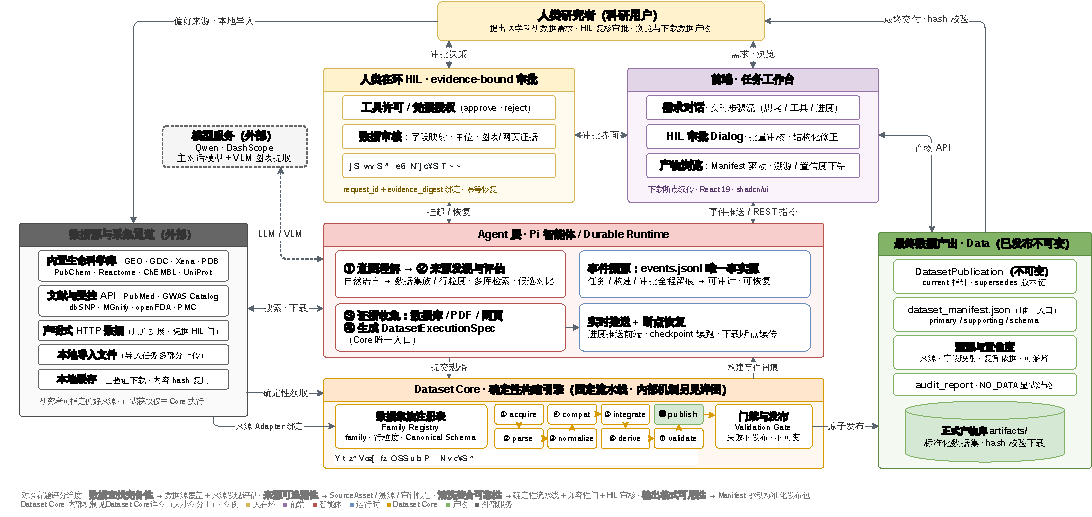
\includegraphics[width=1.00\textwidth]{figures/biomed-qagent-main.pdf}
\caption{\mbox{BioMed QAgent} 主架构。正式写入由 Core 检查；人工验收的请求处理与实际触发情况分别见\ref{sec:hil} 节、\ref{sec:corrected-six-run} 节。}\label{fig:main-architecture}
\end{figure}

\section{系统组成总览}

Dataset Core 负责正式数据处理与发布。其余五部分负责交互、模型调用、任务运行、来源访问和人工确认：

\begin{itemize}
  \item 前端任务工作台：提供需求对话、工具进度、人工确认和发布物浏览。研究者可以查看来源记录、处理过程、检查结果，并下载清单列出的文件（图~\ref{fig:ui-workbench}）。
  \item 模型服务：通过 DashScope 等接口调用 Qwen 主对话模型和视觉模型。模型提出查询、字段映射或变换代码；生成候选文件不等于获得正式发布权。
  \item Agent 层：理解需求、发现来源、收集证据，并向 Core 提交数据集执行规格。运行事件用于记录进度和恢复任务。
  \item 数据源与采集通道：包括 GEO、GDC、Xena、PDB、PubChem、Reactome、ChEMBL、UniProt 等数据库，文献及受控 API，声明式 HTTP 数据源、本地导入与缓存。正式输入需由 Core 获取或登记为任务来源资产。
  \item 人工确认（Human-in-the-Loop，HIL）：处理许可、数据审核与发布验收。审批类型可采用人工审核、模型初审或自动通过；其中要求人工处理的请求不接受模型代审。具体规则见\ref{sec:hil} 节。
\end{itemize}

\begin{figure}[htbp]
\centering
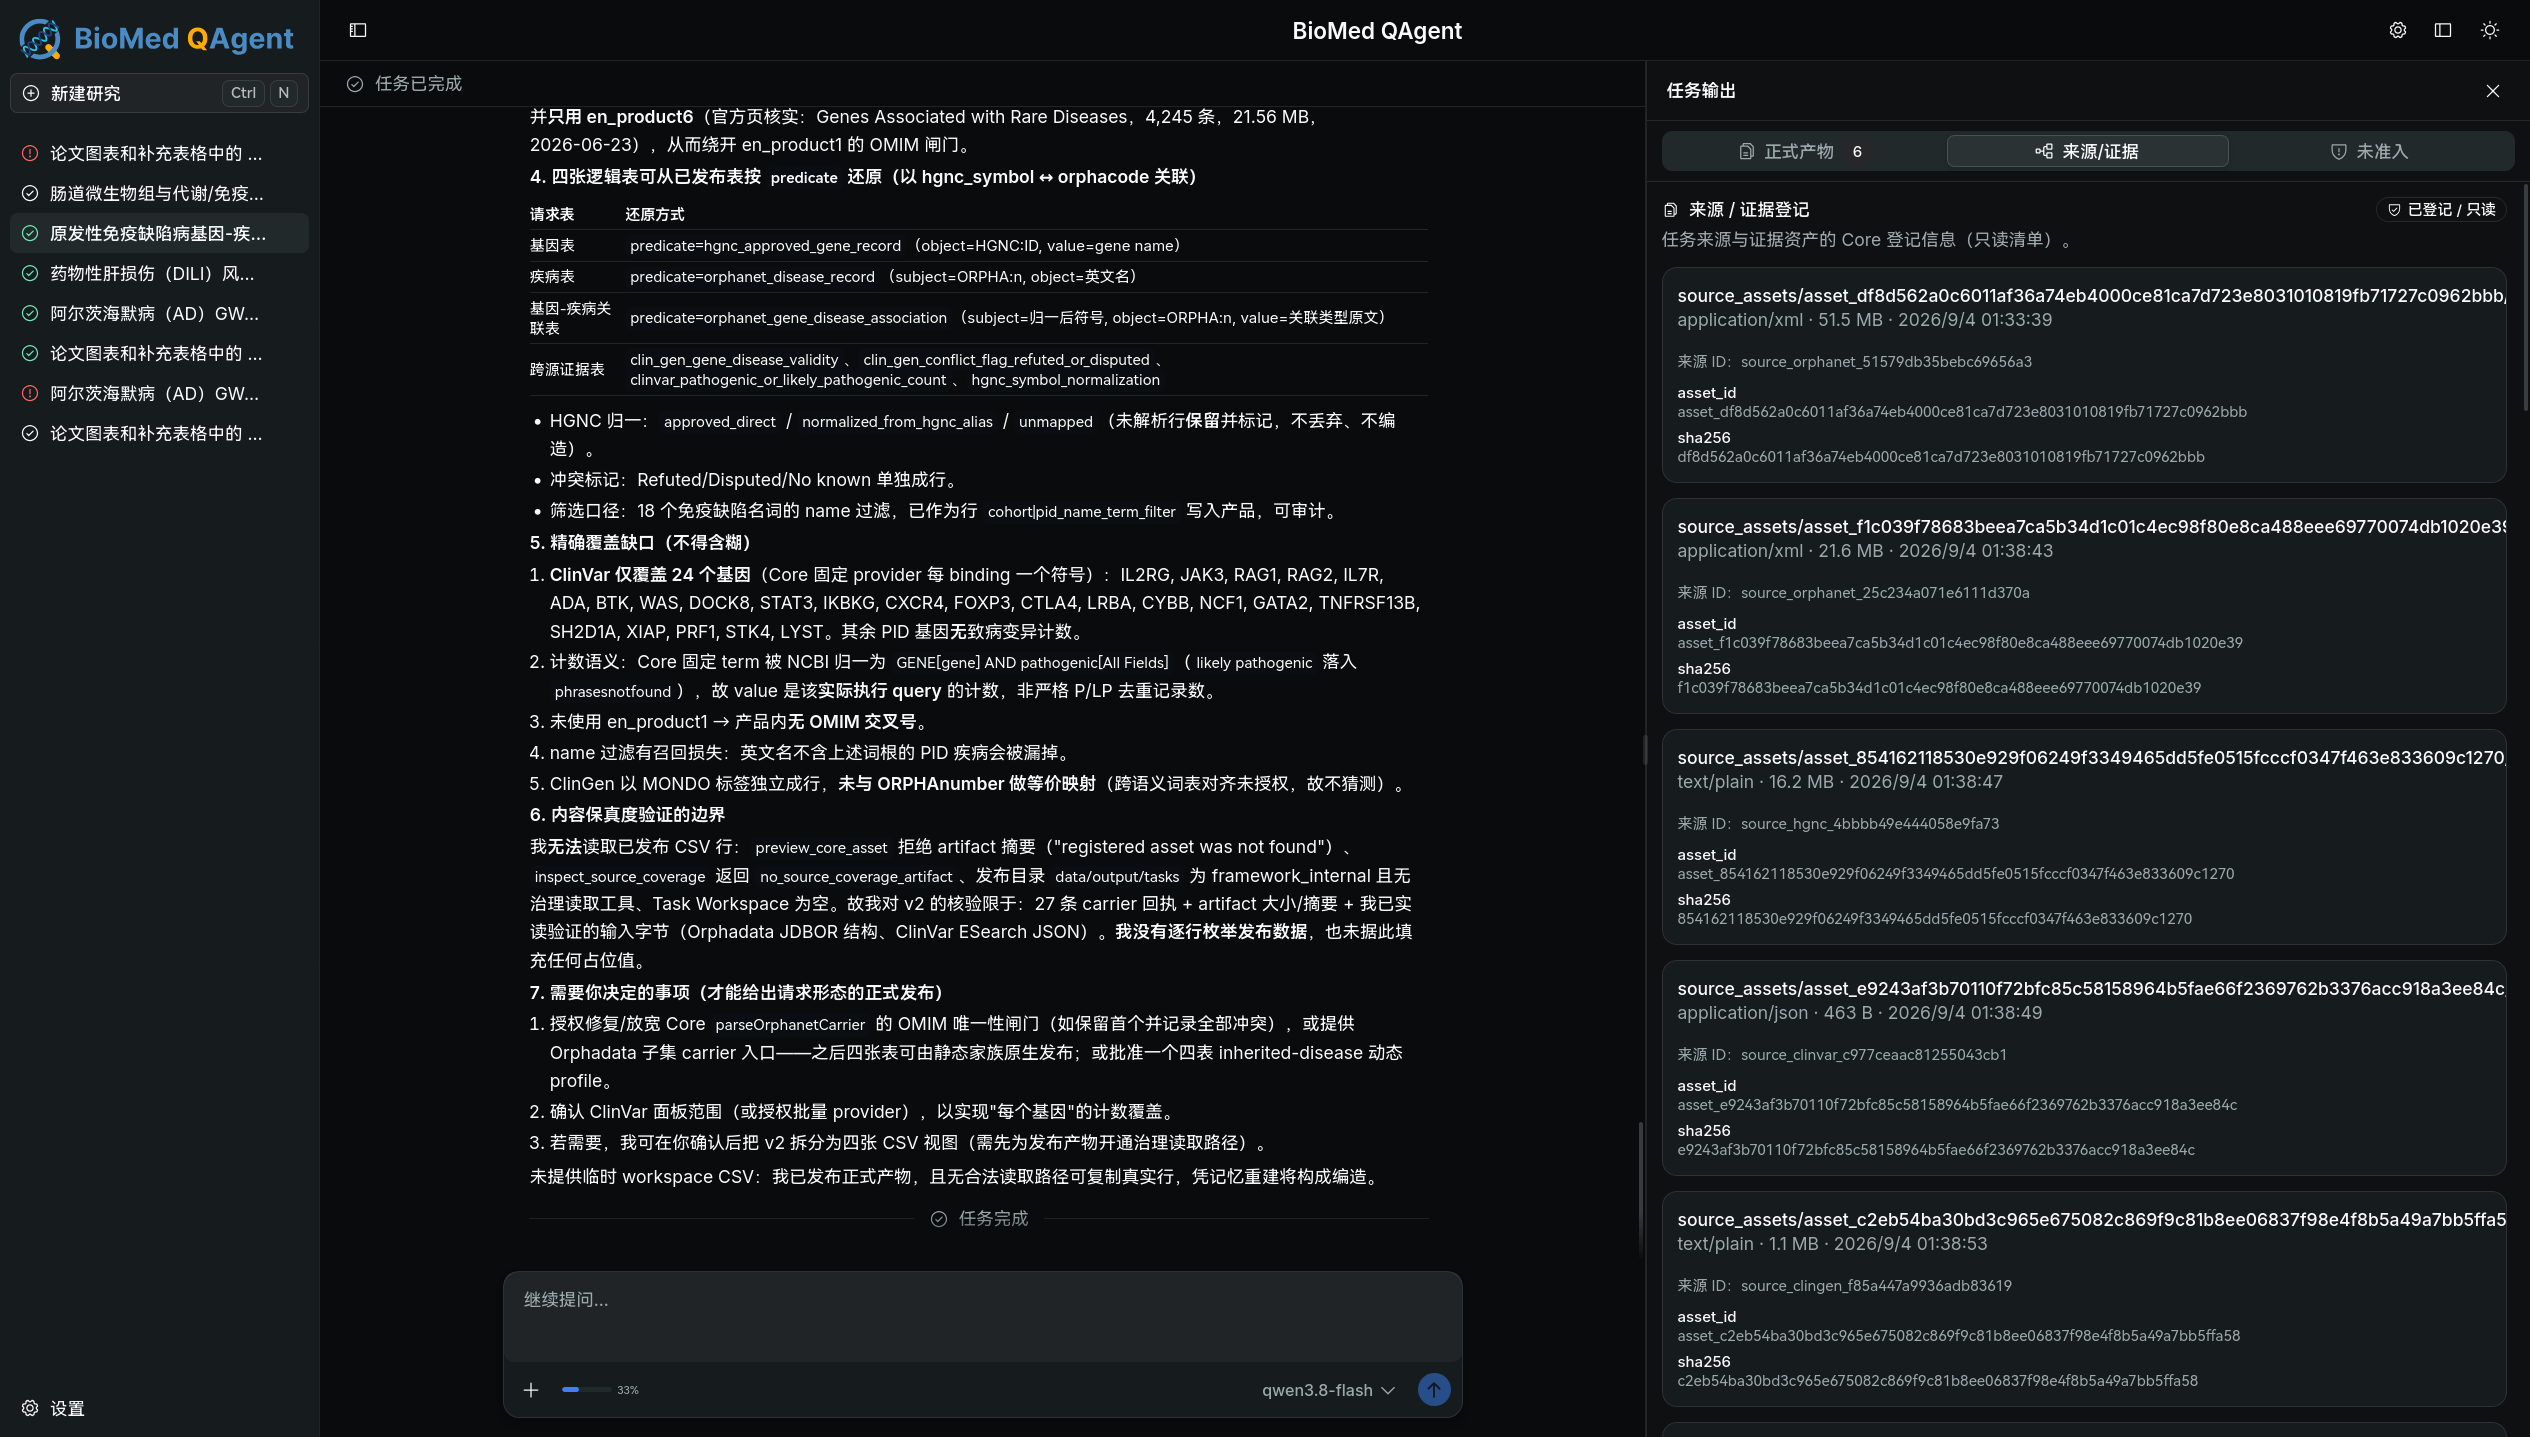
\includegraphics[width=0.90\textwidth]{figures/ui-gold9-source-registry.png}\\[0.4em]
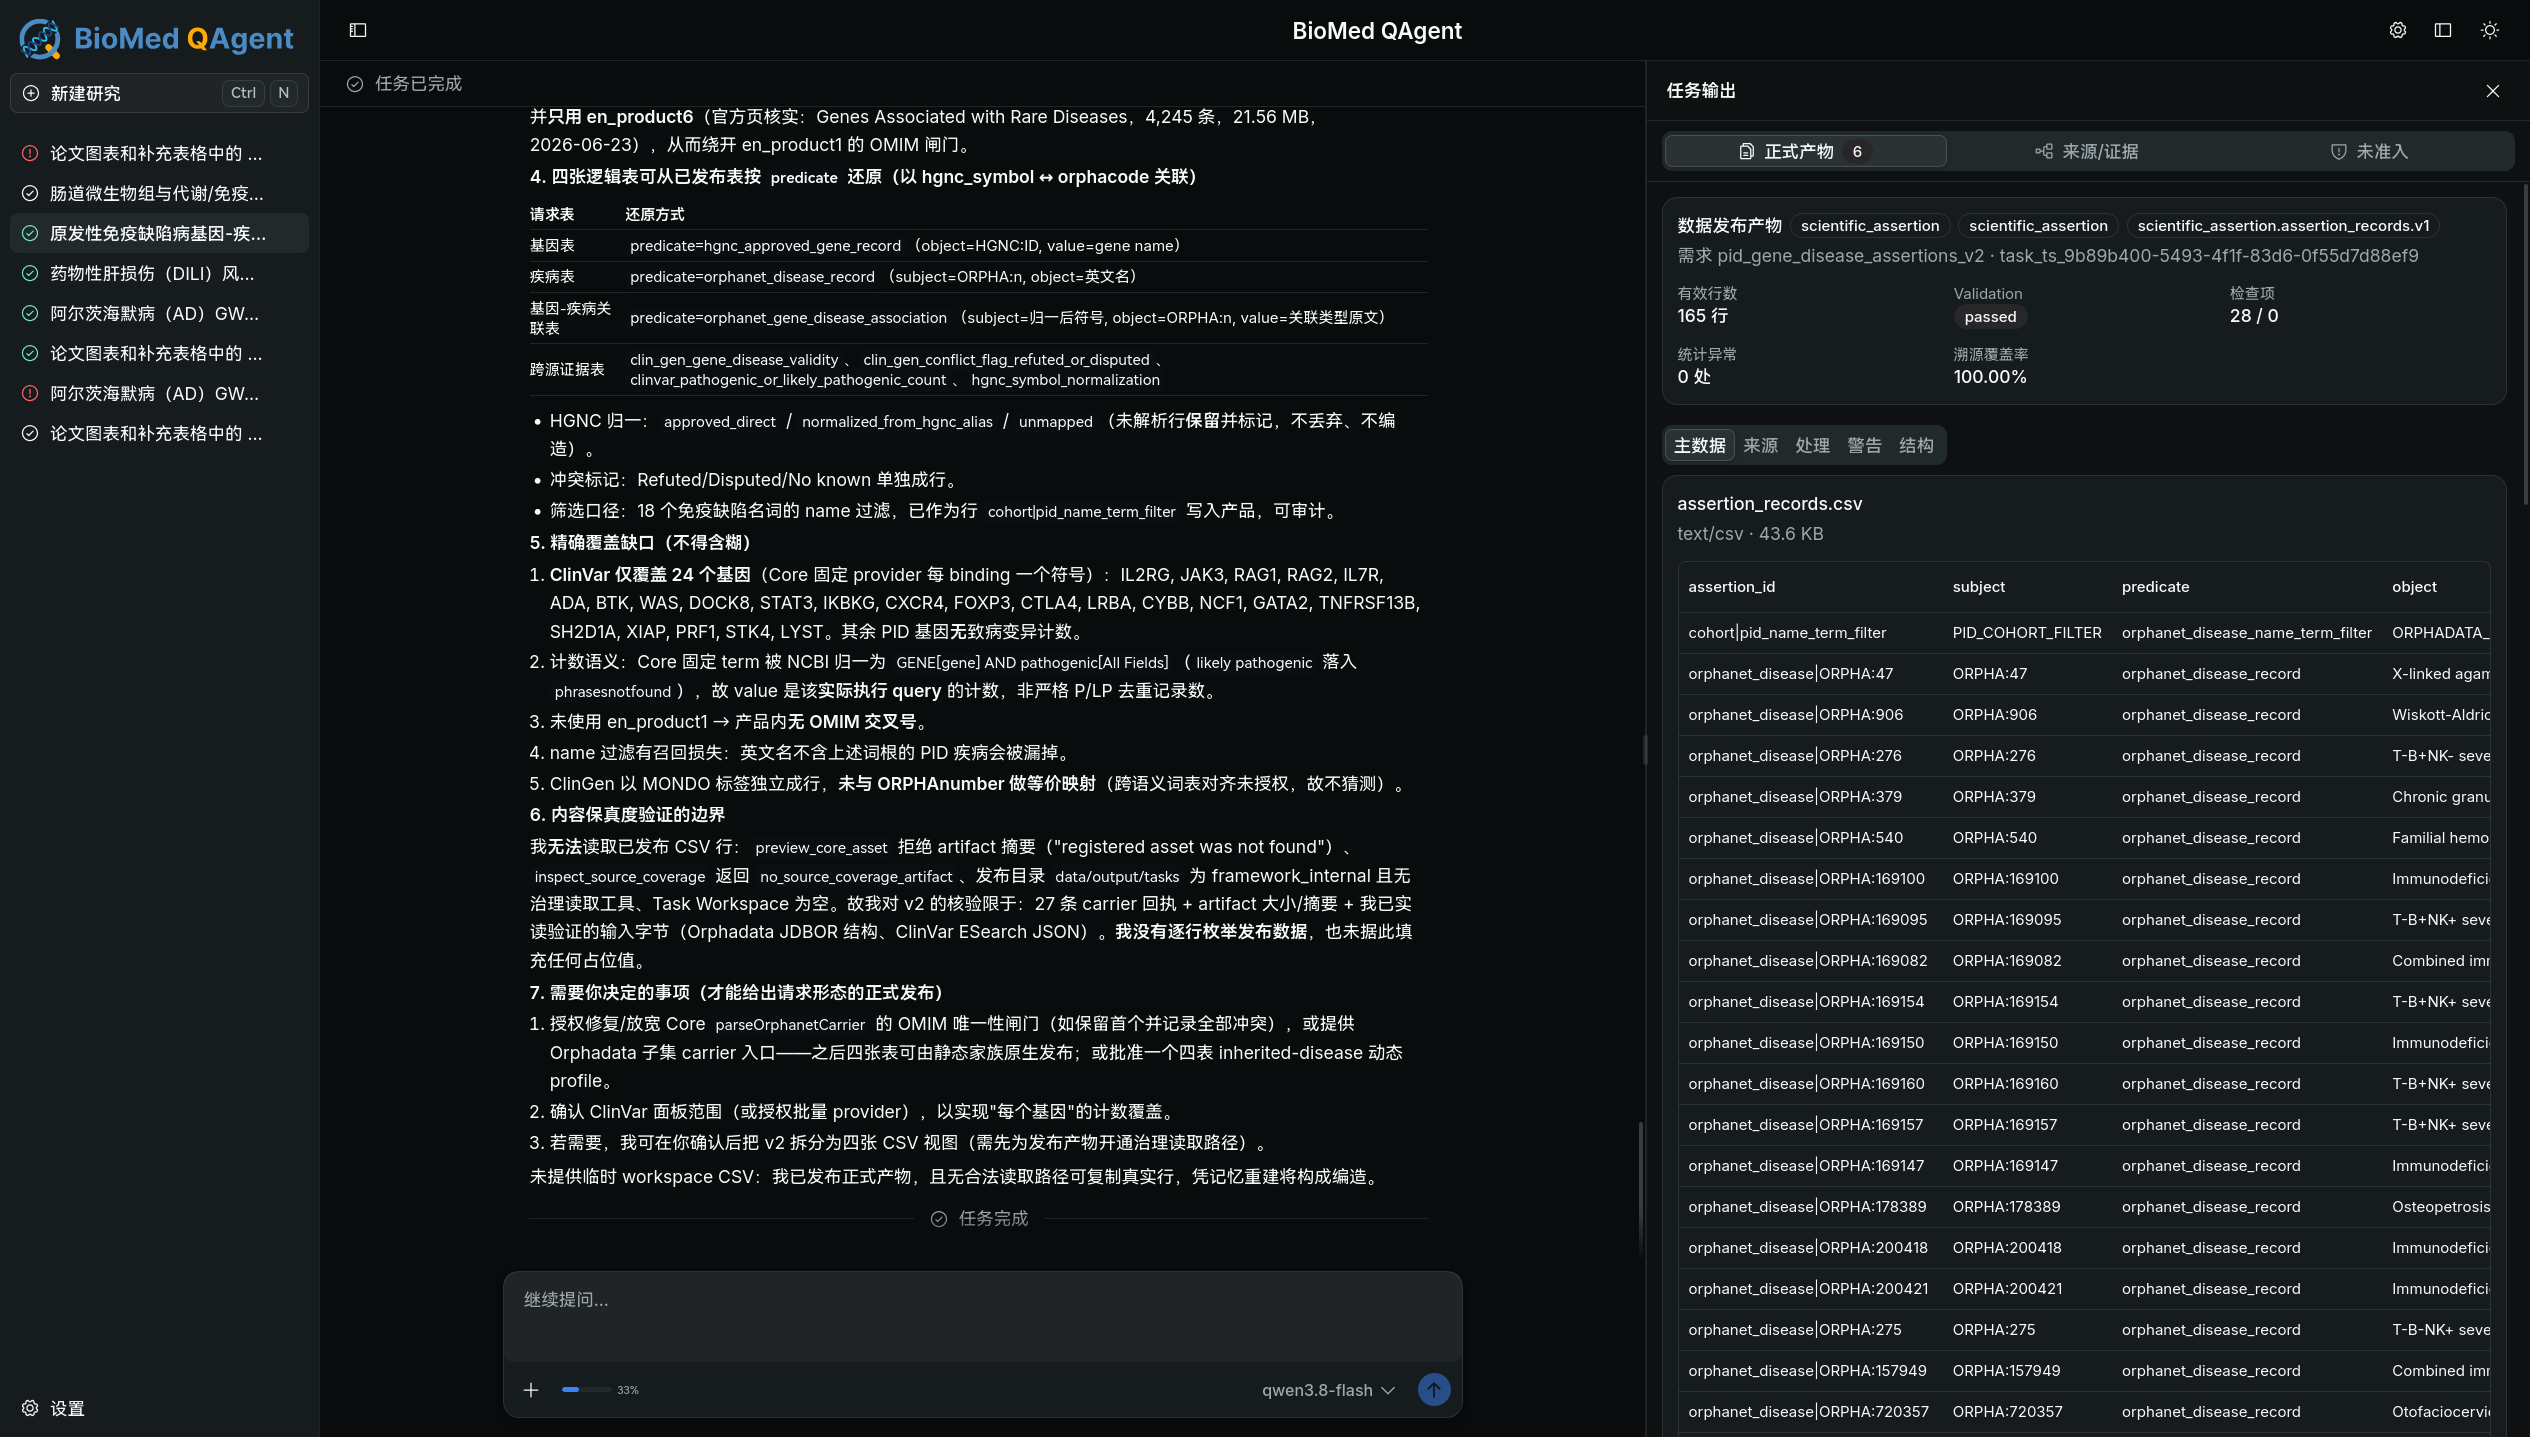
\includegraphics[width=0.90\textwidth]{figures/ui-gold9-artifact-validation.png}
\caption{前端任务工作台。上：来源登记与证据查看；下：发布文件核验与下载。}\label{fig:ui-workbench}
\end{figure}

\begin{figure}[htbp]
\centering
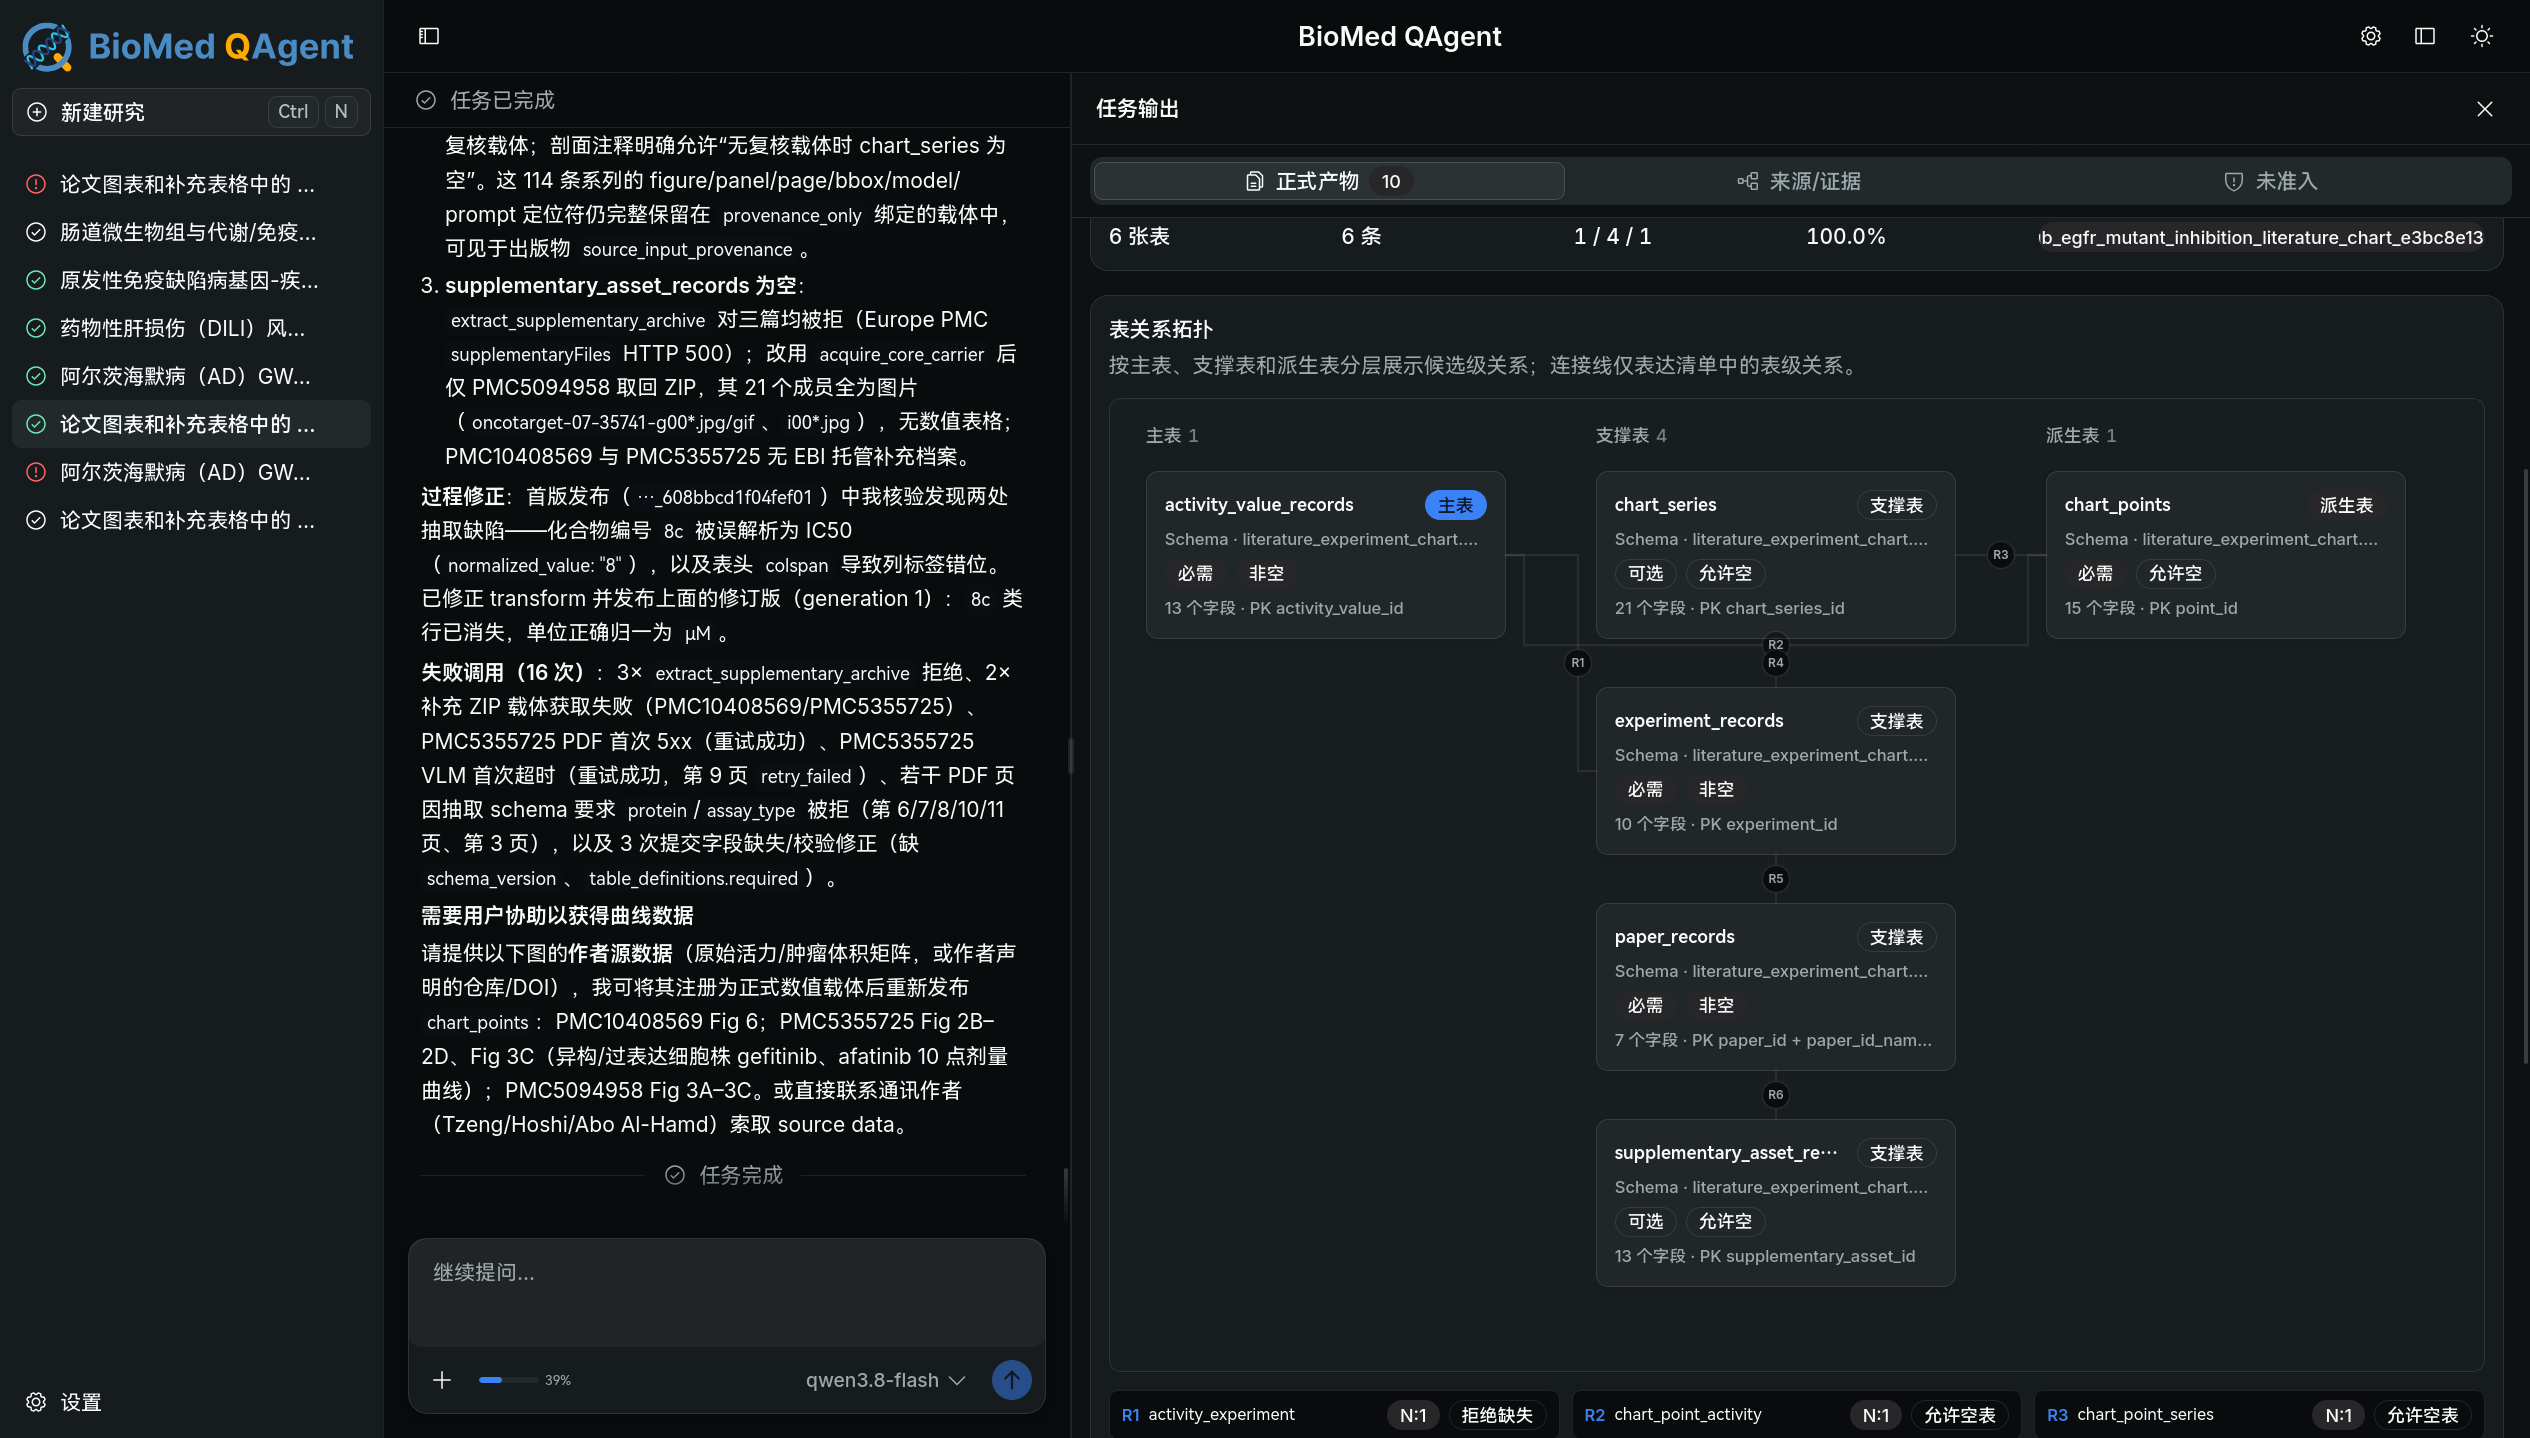
\includegraphics[width=0.88\textwidth]{figures/ui-settings-models.png}
\caption{模型配置界面：可设置模型名称与服务凭据，并单独选择视觉模型。}\label{fig:ui-settings-models}
\end{figure}

\section{三层产物模型}\label{sec:three-layer}

\begin{enumerate}
  \item 工作区暂存结果：搜索下载、模型阅读、探索脚本和临时 CSV 可以辅助任务，但不视为正式交付。
  \item Core 候选结果：来源已经登记，处理步骤有记录，候选表带有表结构、溯源和检查结果；发布条件尚未满足时继续停留在这一层。
  \item 正式发布结果：候选通过发布检查后，系统创建只增不改的发布目录，并记录各文件大小与摘要。读取时再次核验。前端以此标记正式发布成功，同时仍须另行说明需求完成范围。
\end{enumerate}

三层结果分别回答“文件是否存在”“候选是否符合规则”“是否已经正式发布”。工作区允许检索、试算与脚本试错，但仍受文件和工具权限约束；发布检查则决定哪些结果可以正式交付。

当正式采集尚不支持某个来源，而用户已有外部文件时，可将文件上传到任务暂存区，并声明覆盖完整、部分或未知。服务端生成存储标识，计算文件大小和 SHA-256，回执将其标记为不可信参考；下载时重验摘要。该目录与正式发布目录分开，随任务删除。上传回执不能代替来源登记、候选检查或发布许可。

\section{研究需求编译}\label{sec:requirement-compile}

Agent 首先从用户问题中整理出目标实体、数据类型、样本或队列条件、必需字段、期望层级和输出要求。随后，Agent 必须执行一次“路线检查”，确认当前注册表（服务端登记的各项能力清单）支持哪些数据家族、表结构、来源和解析器组合，以及动态路线能够直接绑定哪些数据提供者。

以样例1的“乳腺癌肿瘤与正常组织转录组整合”为例，Agent 需要明确表达表采用探针级还是基因级记录，如何识别样本分组，绑定哪些 GEO 系列与平台注释，以及怎样保存探针—基因对应关系。这些决定写入执行规格，供服务器逐项检查。明确规格并不自动排除遗漏，纳入范围仍须与原始任务核对。

需求编译不是把自由文本简单改写，而是形成数据集执行规格。服务器会交叉校验这份规格：数据家族与表结构是否已注册，行层级与目标实体层级是否一致，每个来源绑定的提供者、解析器和参数是否合法，规范化、合并和校验配置是否在白名单内，输出格式是否受支持，以及多表输入的角色关系是否闭合。任一项不通过，系统都会阻断执行或要求修正。

路线指执行数据构建的固定路径：静态路线使用注册表中现成的数据家族与解析器；动态路线允许Agent为未注册的多表结构临时申请一条受控执行路径。如果注册表能够精确表达需求，Agent 采用静态路线。如果静态结构不匹配，但所有输入都能由Core 的提供者获取（或已经是任务拥有的来源资产），Agent 可以采用动态路线。两条路线都无法闭合时，系统只交付明确标记为暂存的结果，并列出缺失的正式能力，不将其伪装成正式发布。

\section{候选来源发现}\label{sec:source-discovery}

Agent 可以组合文献 API、专业数据库、补充材料归档和网页搜索。文献查询采用主题词与同义词，数据库查询使用实体标识与字段，网页搜索补充预置通道之外的入口。检索结果包括数据集编号、论文、附件、下载地址及其字段和范围。不同通道返回的信息可以互查，但同一来源多次出现不等于增加了独立证据。

来源发现的自主性在样例8 的一次重跑中有直观体现。这次任务（药物性肝损伤）中，官方DILIrank 文件持续返回404，Agent 没有停留在反复重试上，而是经受控浏览器访问搜索引擎结果页，从命中记录中找到LiverTox 官方通道，先后完成16 次页面读取与13 次取证下载，并对5 组openFDA 不良事件查询作交叉核对，全程没有请求权限，也没有人工提示。与之配套的是止损规则：浏览器通道对同一主机的连接性失败连续达到阈值即短路，返回结构化的“无数据”信号。早期运行曾观测到对同一失效地址连续555 次顺序枚举的空转，这条规则就是为了阻断这类行为。

Core 按规格中的来源绑定记录检索计划与采集结果。记录包括查询参数、采集回执、解析与保留行数、拒绝及排除原因、请求上限，以及成功、失败、尚未尝试的来源数量。Agent 可以据此调整查询或补充来源，避免将失败来源从最终说明中省略。

来源覆盖统计只回答“计划中的来源处理了多少”。未纳入计划的数据库、未发现的附件不在分母内，因此该比例不能代表问题子领域已经查全。计划外遗漏需要用独立整理的参考来源集合核对。预置通道之外的材料可以经声明式 HTTP 接入、浏览器取证或任务上传进入系统；正式采用前仍需登记来源并接受检查。

\section{Agent 的自主决策面}\label{sec:agent-autonomy}

Agent 与Core 的分工可以概括为：Agent 负责开放式的研究决策，设计数据产品；Core 负责按确定性规则实现设计，并验证其是否可以交付。Agent 的自主性体现在数据产品生产的各个决策点上（表~\ref{tab:decision-inventory}）。Core 约束的是这些决策进入正式数据的通道，而不是决策本身。Core 拒绝的是执行期的任意DAG 编排：Agent 不能提交自定义的处理节点链、合并函数或发布路径。数据模型层面的多表拓扑设计（表、主外键与角色映射）属于Agent 的决策面，二者分属执行编排与产品结构两个层面。

\begin{table}[htbp]
\centering
\caption{Agent 的自主决策清单}\label{tab:decision-inventory}
\begin{tabularx}{\linewidth}{>{\hsize=0.40000\hsize}L>{\hsize=1.30000\hsize}L>{\hsize=1.30000\hsize}L}
\toprule
\textbf{决策点} & \textbf{Agent 自主决定} & \textbf{Core 的约束} \\
\midrule
检索与来源 & 组合查询、比较候选、决定采集对象和顺序 & 正式输入需由注册提供者获取或登记为任务来源资产 \\
执行路线 & 选择静态路线，或提出表、主外键、角色映射与来源绑定 & 规格先检查，候选文件逐件重新计算摘要 \\
规格迭代 & 依据错误说明修正表结构与参数 & 逐字段返回拒绝原因；不通过则不执行 \\
质量与修正 & 决定补源、修改规格、重新提交或说明未完成部分 & 新发布保留旧文件；已触发的审批按规则处理 \\
数据值 & 提出字段映射、单位换算和抽取候选 & 候选必须经过准入、完整性检查、产品评估与发布检查；检查不等于自动证明数值正确 \\
\bottomrule
\end{tabularx}
\end{table}

\section{LLM 使用方法与上下文工程}

本节说明Dataset Core 之外的Agent 侧如何使用LLM 以及如何组织上下文，对应\ref{sec:contributions} 节的贡献一。证据上下文控制（\ref{subsec:evidence-context} 节）与第第\ref{ch:dataset-core}章的确定性校验上限和人工确认机制直接衔接。

\subsection{完成规则与运行状态注入}\label{subsec:completion-contract}

系统提示要求 Agent 区分正式发布和任务完成。数据生产请求只有取得本次运行的正式发布物及其清单，才可报告“发布成功”；仅有临时 CSV 或自写文件清单不满足这一条件。报告还须说明已交付与未交付的任务条目，不能因某个较小规格执行成功而宣称原任务全部完成。

完成判定也有提示词之外的支撑。运行时每回合都会注入一条由事件流压缩而成的运行状态，内容包括当前阶段（规划/执行/等待工具/收尾）、工具调用的成败计数、是否已存在不可变发布物，以及下一步建议，例如“仍有N 个工具在执行，不要假定其结果”，或“最近一次失败为某工具，仅在可重试或换用独立来源时重试”。这样，完成与否以数据产品的实际状态为依据，而不是以模型对自身行为的记忆为依据。

\subsection{行为约束：从实测失败模式到提示规则}\label{subsec:behavior-rules}

系统提示词中的行为约束来自对模型失败模式的实际观察。开发期在同一个表达组学案例（乳腺癌GEO 表达整合）上的提示词迭代记录显示，轻量模型在无人工干预的长流程中反复出现三类行为偏差。其一，时限幻觉：某次运行在240 回合的预算仅使用35 次模型调用时，以“由于时间限制和复杂性”宣布放弃并等待用户指示，而系统从未设置任何时限。其二，重复失败：对同一数据集以同一套参数连续失败七次，仍不改变策略或换用其他来源。其三，发布后反复自检：正式发布完成后，模型反复重读已经验证过的回执，一次运行中这部分重复验证消耗了全部计费token 的79\%。

系统提示词针对这三类行为逐条写入了约束：声明系统不以未经配置的总时限为放弃理由，回合与上下文预算只是防止失控的上限，不允许以时间限制为理由放弃任务；同一错误重复出现时，立即停止同形态重试，改为查清被拒绝的具体原因，或换用真正独立的来源；每件发布产物只验证一次，验证后记录结论并转入最终报告。决策方式也作了相应调整：不确定某个工具或检查如何运行时，直接阅读它的实现源码，以代码为准判断“接受什么输入”，而不是凭记忆反复试错。

在一组前后对照的迭代中，同一案例、同一模型、同一任务的工具调用从60 次降到36 次，计费token 从5.71M 降到3.73M，工具错误从7 次以上降到2 次。迭代中也识别出一些值得保留的行为模式，如单平台同粒度设计优先、拒绝跨研究拼接行、发现映射未经验证时主动修订而不是宣称完成；这些模式随后写入流程技能，成为后续运行的默认规则。该迭代发生在第五章评测之前，用于校准提示词，不计入评测结果。

\subsection{路由预检与声明式工具结构描述}

\mbox{BioMed QAgent} 向大模型公开当前真实能力及相关参数。静态路线要求精确匹配注册表中的数据家族、表结构与来源能力清单；动态路线只接受预检报告确认可以绑定的输入。工具参数的结构描述严格约束字段类型、枚举、对象结构和必要参数，服务器端还会进行交叉验证。

上下文工程的重点不是把所有代码放进提示词，而是提供模型决策所需的最小必要信息。这些信息包括：当前任务与研究目标，可用工具及其严格输入结构，注册表返回的数据家族、表结构和提供者能力，来源搜索结果与失败回执，校验问题、人工确认选项及证据摘要，以及当前发布物或阻塞状态。这样可以把“模型知道什么”绑定到运行时的实际能力，减少提示词与代码版本之间的漂移。

\subsection{技能体系与专用工具}\label{subsec:skills}

专用能力按数据库访问、载体取证和任务流程三类组织。技能描述入口、查询方式、字段含义和使用步骤，工具执行具体操作；其结果是否可以正式采用，仍由 Core 检查。

其一，数据库类技能14 项：PubMed、GEO、GDC、Xena、UniProt、PDB、PubChem、ChEMBL、ClinVar、GWAS Catalog、dbSNP、MGnify、openFDA、Reactome——每项封装对应入口的查询、分页与来源特有字段，Agent 不必为每个站点编写脚本。

其二，载体与取证技能：包括浏览器导航与页面取证、PDF 表格提取、图表视觉提取（qwen3.8-flash）、文献理解、网页视觉取证、搜索发现和本地缓存复用。

流程类技能包括数据集构建引导、研究数据指引和分析。构建引导要求先检查执行路线，再编写与校验规格，最后核对正式发布物；研究数据指引说明如何选择来源、清洗数据并记录未查来源。分析技能可以辅助查看结果，但不取代正式数据发布，也不代表系统已经验证科学结论。

在已有访问方式和解析器能够处理目标数据时，可以通过声明式配置扩展来源。新协议或新格式仍需补充相应代码。工具返回结构化结果与错误，供 Agent 调整查询或说明缺口；新增技能不会绕过网络权限、来源登记与发布检查。

\subsection{证据上下文与不确定性控制}\label{subsec:evidence-context}

模型不应仅看到最终值，还应看到该值的来源类别、定位信息、解析层级和置信度。对于非确定性抽取，系统记录该值的置信类别、给出该类别的理由、执行抽取的模型与其提示版本、以及是否经过人工复核，并在Core 中设置可信度上限。

模型提出字段映射、单位修正或抽取值时，应同时说明依据。正式采纳取决于注册规则、候选检查和必要的人工决定。证据类型分级用于安排检查，不应写成经过统计校准的正确概率。


\chapter{确定性数据核心：八阶段流水线（Dataset Core）}\label{ch:dataset-core}

Dataset Core 是系统唯一的数据信任边界。它将数据处理固定为八个阶段：采集、解析、规范化、兼容性检查、整合、多表组装、校验、发布。每个阶段都有明确的输入、输出摘要和执行凭证，记录该阶段产生了哪些文件及各文件的摘要。本章按阶段说明各环节对数据质量的实际作用。

\begin{figure}[htbp]
\centering
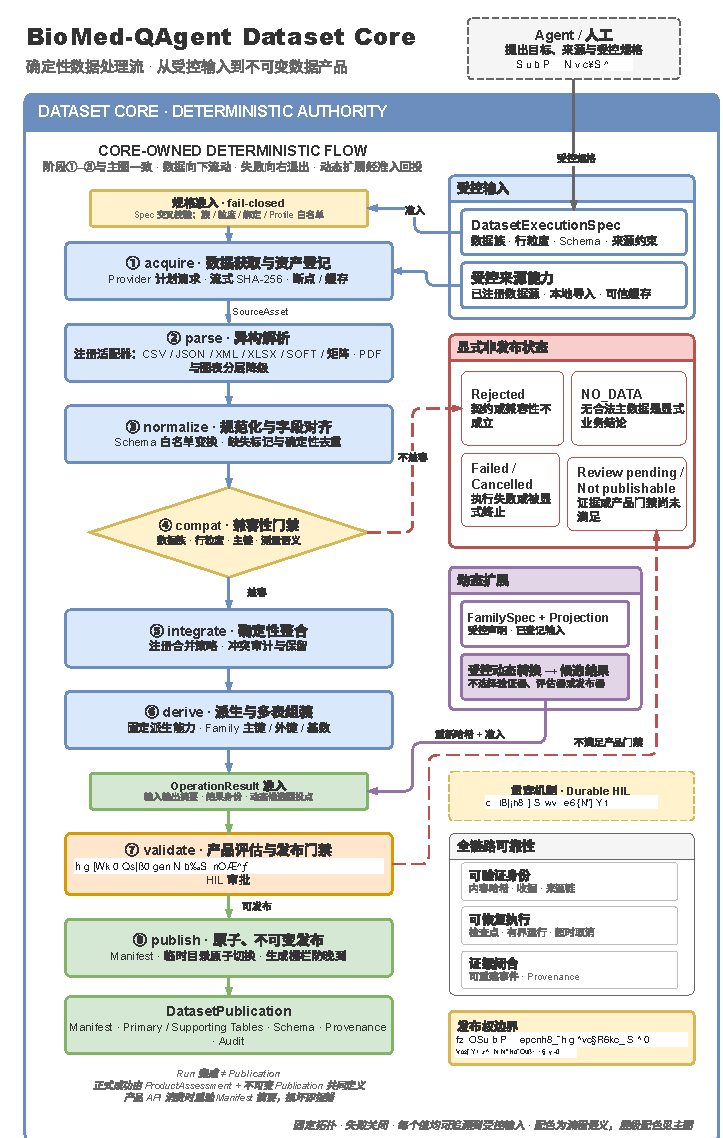
\includegraphics[width=0.66\textwidth]{figures/biomed-qagent-core-deterministic-flow.pdf}
\caption{Dataset Core 数据流。候选文件先接受检查，再进入正式发布；审批按请求类型执行。}\label{fig:core-deterministic-flow}
\end{figure}

Core 采用固定处理顺序，但输入与变换方案可以变化。静态路线使用已注册的数据家族；动态路线允许 Agent 提出多表结构和变换代码，先产生候选文件，再交给 Core 检查。变换方不能自行选择验证器、评估器或发布器。这里分开的是候选与正式文件，并不声称具备操作系统级沙箱隔离。

准入检查核对输入来源、输出表头和摘要是否与声明一致。例如输出列与声明不符时，系统返回 OUTPUT\_HEADER\_MISMATCH。通过这些检查仍可能存在计算或字段含义错误；这类问题需要审查变换方法并核对原始记录。开发记录也曾出现占位符文件通过旧检查的情况，因此不能从检查全部通过推导出数据必然正确。

Rejected、NO\_DATA、Failed 与 Cancelled 表示不同的非成功结果；等待审核也不等于已经发布。只有满足发布条件，系统才创建正式发布物。

\section{阶段1：正式采集与来源资产登记（acquire）}

Agent 的来源发现拿到URL 后，正式路线不会直接信任工作区中的任意文件。Core 的统一下载设施按预定的请求定义执行网络访问，实施访问策略、大小与超时限制、重试、断点续传和内容缓存。文件写入任务专属目录后，来源资产注册表流式计算SHA-256，把任务、来源身份、内容摘要、媒体类型与采集实现身份绑定为一份输入证据，支持时还记录快照或修订号等版本信息。因此，“来源资产”不是一个本地路径，而是可复核的输入证据。

\section{阶段2：异构数据解析（parse）}

正式静态路线使用已注册的解析器，把来源特有的CSV、JSON、XML、XLSX、SOFT、矩阵或API 响应转换为数据批次，同时输出解析统计、被拒绝的记录和溯源定位信息。解析器的原则是失败而不猜测：遇到来源格式异常时，解析器应失败或将问题写入审计记录，而不是让模型猜测缺失字段。

表达数据的解析集中体现了行层级纪律。GEO 既可能提供基因级结果，也可能只提供探针级矩阵；系统不会在缺少可信注释时把探针当成基因，一行究竟代表一个探针还是一个基因由表结构显式声明。GDC 与Xena 的输入形态不同，但都必须转换到目标表达表结构后才可合并。

论文衍生的载体单独处理。PDF 表格解析保留页面与位置证据（页码、边界框、题注），无框线表格与跨页表头仍是启发式解析难点，这类解析结果需人工核对。图表走视觉模型通道（4.2.1 节）。

\subsection{图表与视觉模型}\label{subsec:chart-vlm}

图表工具优先调用 qwen3.8-flash 读取页面或嵌入图像；调用或解析失败后，尝试 PDF 表格解析，再失败则仅保留图表标题。视觉提取只转录图内明确印出的数值，不将曲线像素位置估算为精确原始值。没有数值标注时，Agent 应继续检索正文表格、补充材料、出版社 source data 或作者仓库；仅识别曲线和描述趋势不计作数值数据交付。格式正确但数值错误的回答不会自动触发降级，仍需与来源核对。

VLM、PDF 表格或标题抽取结果先形成带来源定位的图表证据，再由数据家族组装。每个数据点记录抽取模型、置信度及其依据；人工修正保留原值和修改记录。样例6发布了六张关联表与三件说明文件，但存在这些文件并不等于图表数值已经完整取得；该案例的交付比较见\ref{subsec:gold6-artifact-compare} 节。

图系列表记录轴名、单位、刻度和图例，并声明含义明确、含义不明或已经人工确认。规则检查声明与点数据是否矛盾：例如标为“精确”的点不能同时对应含义不明的轴。轴状态若从一开始就误报为明确，此类一致性检查无法发现错误。因此，本文将其称为图表证据一致性检查，不等同于独立识别全部坐标轴或图例解析错误。点级样例测试只能证明相应检查路径可以执行，本轮尚未报告端到端数值误差率。

\section{阶段3：含义规范化与缺失、重复处理（normalize）}

规范化器依据目标表结构完成类型转换、字段命名统一、实体标识表达和必要的值标准化。核心原则是：只有目标表结构和规范化配置明确授权的变化，才可以自动执行；规范化过程保留原始写法与规范值之间的血缘，便于任何一处转换被事后复核。

缺失与重复按类型分层处理：必填字段缺失时拒绝或阻断，可选字段缺失保留为空并计入完整性统计；完全重复按确定性键去重；主键重复且值一致时合并血缘、保留多来源。每类处理都保留对应证据，以便后续复核。

实体身份对齐同样采用确定性机制：化合物以InChI Key 精确匹配建立交叉映射表，匹配不上时显式标记为冲突而不强行合并；基因符号归一使用内置确定性映射表；探针到基因的映射依赖逐平台注释资产，未映射探针保留原命名空间，不静默丢弃。这些注释资产与来源文件同样按内容摘要登记，映射结果随发布件交付。

\section{阶段4–5：兼容性检查与多源整合（compat、integrate）}\label{sec:stage5-integrate}

解析与规范化产物进入整合前，兼容性检查核对各批次在数据家族、表结构、行层级、实体层级、单位、含义和尺度上是否可以合并，并据此生成确定性的合并域键：值的含义、尺度与单位，加上物种、特征命名空间、测量类型、规范化状态与参考版本等维度，任何一维不一致都不能进入同一合并域。未知单位或不受支持的数值尺度不会被自动修正；单位换算只在有注册转换公式时执行，公式限定为线性安全形式，没有注册规则时阻断或交人工选择，系统不会自动“猜”一个换算。

整合器按注册策略合并批次。主键相同且数值一致时，保留多来源记录；数值冲突时，记录冲突键、双方取值与保留结果，必要时停止发布。采用先到优先处理同键冲突时，重跑也需要固定来源处理顺序。这种取舍使结果可以核对，并不说明先到来源更可靠。研究者可以根据证据重新判断，修正后另行发布。

\section{阶段6：多表组装（derive）}\label{sec:stage6-derive}

对于需要关联多个实体的数据，组装阶段生成多表候选，检查主键、外键、基数和表角色。\footnote{主键标识一行；外键指向另一张表的主键；基数说明两表记录是一对一、一对多还是多对多；表角色说明某张表记录测量值、身份信息或其他内容。}

单表与多表由数据关系决定。一个观测层级可以使用单表；测量值、实验条件与化合物身份需要分别保存时，再拆成关联表。生物活性表 activities 通过外键关联 assays 与 compounds，并辅以靶点、来源和交叉映射表（图~\ref{fig:bioactivity-fk}）。发布清单声明连接键与关系，下游无需根据同名列猜测如何拼接。

\begin{figure}[htbp]
\centering
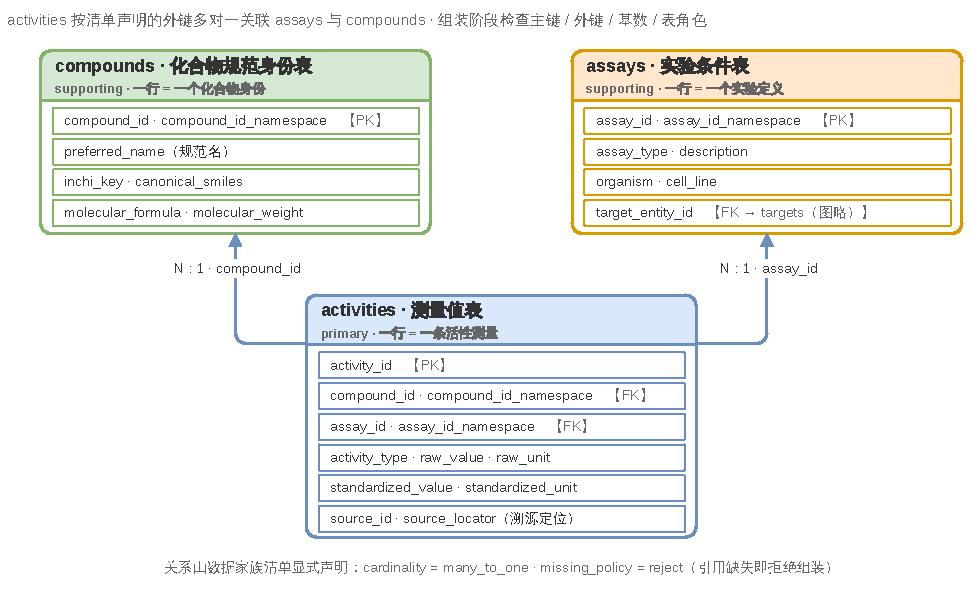
\includegraphics[width=0.94\textwidth]{figures/biomed-qagent-bioactivity-multitable-fk.pdf}
\caption{生物活性多表关系：activities 通过外键关联 assays 与 compounds。}\label{fig:bioactivity-fk}
\end{figure}

\section{阶段7：校验、置信度与产品评估（validate）}\label{sec:stage7-validate}

发布前检查字段类型、必填项与允许缺失率、主外键、实体命名空间、单位、来源定位、置信度记录，以及文件摘要和处理版本。多表产品评估从结构、关系、标识、溯源、置信度和复现所需信息六方面记录问题。没有阻断项时判为可发布；仍缺复现信息时，不能取得同等发布评级。这些规则检查文件是否符合声明，不能仅凭通过检查就认定科学含义全部正确。

置信度按证据类型分级。受版本约束的确定性解析可以取得 high；VLM、LLM、OCR 与网页抽取最高为 medium。该分级不是统计校准后的正确概率。本系统不会自动对全部 medium 记录发起人工审核；是否逐点复核与整个产品是否需要发布验收属于两项不同决定。未逐点复核的数值仍需对照原始来源，本轮没有测量各等级的实际错误率。

验证结论与明确的结束状态绑定。空主数据、兼容性失败或验证失败的结果一律不可发布；“运行完成”也不等于“发布物生成”。

\section{阶段8：不可变发布与消费时重验（publish）}\label{sec:stage8-publish}

发布器把质量检查合格的候选复制到独立目录，生成发布清单，逐文件记录相对路径、媒体类型、字节数和SHA-256；发布经临时目录原子切换完成，执行锁与代次围栏保证超时或已取消的旧执行不能晚到覆盖新结果。产品API 在每次读取时重新核验清单与文件摘要，文件被改动或损坏即拒绝展示。这里的“不可变”是应用层语义：正常API 只追加发布、不覆盖旧版本；系统不提供抵御同一操作系统账户重写文件系统的密码学防篡改能力。

\section{持久化人工确认与可恢复执行（Durable HIL）}\label{sec:hil}

字段映射不明确、单位未知、图表点置信度低或冲突无法按规则处理时，系统可以暂停并发出结构化请求。请求列出候选值、置信度、相关记录、证据摘要，以及任务、运行与需求身份。人工可以通过、拒绝或修正。恢复前必须核对请求是否仍有效、对象是否仍与审批证据一致；正常响应晚于请求发出时间，并不是拒绝恢复的理由。

请求分为工具许可、数据审核和发布验收。普通请求可按类型采用人工审核、模型初审或自动通过；模型初审不通过或调用失败时回退人工。对已经发起且属于强制人工类型的请求，非人工审批配置不被接受，只有人工处理后才继续。这个设置约束不单独证明每条动态发布路径都会触发验收：第五章样例7、样例9的归档运行没有业务 HIL 请求，因此本轮不能用它们证明动态发布一律经过人工确认。

\section{可靠性基座}\label{sec:reliability-base}

各阶段共用执行锁、取消检查、事件记录和文件重验。表~\ref{tab:reliability-base}区分设计约束与本轮可观察结果，避免将某次成功运行视为全部故障路径均已验证。

\begin{table}[htbp]
\centering
\caption{运行保护与检查依据}\label{tab:reliability-base}
\begin{tabularx}{\linewidth}{>{\hsize=0.60000\hsize}L>{\hsize=1.10000\hsize}L>{\hsize=1.30000\hsize}L}
\toprule
\textbf{措施} & \textbf{检查或控制的内容} & \textbf{依据与范围} \\
\midrule
执行锁 & 同一任务、同一需求不能并发写入同一发布目标 & 设计约束；并发行为需由专门测试检查 \\
代次围栏 & 发布前核对本次执行是否仍拥有写入权 & 用于阻止超时或取消后的旧执行继续发布 \\
超时与取消 & 操作有界；发布前检查取消状态 & 不能仅凭一次正常运行验证全部取消路径 \\
事件日志 & 追加操作与状态变化，供恢复与核对 & 本轮据事件起止时间和终态整理运行记录 \\
持久化人工确认 & 保存请求和决定，按原调用恢复 & 样例6记录了许可与发布验收；详见\ref{sec:hil} 节 \\
文件摘要与重验 & 读取时重算文件摘要，与清单比对 & 验证文件与回执一致，不验证重跑或科学正确性 \\
\bottomrule
\end{tabularx}
\end{table}


\chapter{实验与评测}\label{ch:experiments}

本章检查系统能否形成正式数据产品、能否保留来源与处理记录，以及与通用智能体环境相比交付了哪些内容、花费多少时间和模型用量。实验包括十案例汇总与两个案例的跨环境观察。每个列示条件只有一次运行，不据此估计稳定成功率，也不作单项机制的因果判断。

\section{评测问题与方法}\label{sec:eval-protocol}

十个案例覆盖表达组学、变异、靶点证据、蛋白结构、生物活性、论文图表、GWAS、药物安全、罕见病和微生物组。系统接收研究任务，记录起止时间、模型用量、工具调用、人工确认与终态。一次任务提交到终态计为一个运行单元，内部重试不另计。本文汇总不同批次的十二次运行，不将其写成同一代码和提示配置下的统一试验。

其中，样例6—10的 flash 运行与样例6的 max 运行来自已归档的六运行批次，使用代码提交 \code{e5aadfe0}\cite{biomed-evidence}。样例6使用冻结的任务与执行上下文；样例7、8、10使用重建的历史任务提示；样例9从历史事件恢复原始输入。样例6 max 的完整标识为 \code{qwen3.8-max-0902}，并使用修正模型元数据后的代理运行环境。以上差异保留在运行记录中，不归因于模型档位本身。

评测分开记录三类结果。正式发布状态说明文件是否通过配置的发布检查；需求完成情况说明原始任务中哪些内容已经取得、哪些仍有缺口；运行成本记录时间、token 和工具调用。来源标注、记录定位、清单、方法、质量检查及原始材料则用于判断结果能否进一步复核。文件摘要一致只说明交付文件与记录相符。

十个案例各列示一次 qwen3.8-flash 运行，样例1与样例6另列一次 max 运行。样例1的两个环境做过共有记录抽样互查，但未对照原始来源。本轮没有给出来源级数值正确率、独立参考集召回率或冻结输入后的重跑一致率；这些指标不能由发布率或哈希通过率代替。

\textbf{实验材料。}六运行批次的起止事件、token 分项、工具计数和发布摘要见仓库 \path{docs/evaluation/gold6-10-2026-09-03/}；Qoder 样例6离线包的复核结果见 \path{docs/evaluation/gold6-qoder-2x2/}。这些材料支持各自范围内的核对，不包含全部跨环境计时和用量原始记录。Qoder 时间与 token 沿用人工记录，仅作为描述值保留，不据此计算费用或声称同等工作量下的效率收益。

\section{十案例总体表现}\label{sec:gold-overview}

\subsection{完成情况与数据产品}

表~\ref{tab:gold-overview}汇总每个案例的 flash 运行。样例1—9至少形成一次正式发布，样例10因必需数据未满足条件而停止。表中“成功发布”是运行状态，不表示原始需求全部完成；多次发布与多件文件也不重复计为成功案例。

\begin{xltabular}{\linewidth}{>{\hsize=0.43000\hsize}L>{\hsize=1.25000\hsize}L>{\hsize=0.67000\hsize}L>{\hsize=1.78000\hsize}L>{\hsize=0.87000\hsize}L}
\caption{十案例运行结果与实际交付内容}\label{tab:gold-overview}\\
\toprule
\textbf{案例} & \textbf{研究任务} & \textbf{发布状态} & \textbf{已交付内容与范围} & \textbf{时长 / token} \\
\midrule
\endfirsthead
\toprule
\textbf{案例} & \textbf{研究任务} & \textbf{发布状态} & \textbf{已交付内容与范围} & \textbf{时长 / token} \\
\midrule
\endhead
样例1 & 乳腺癌肿瘤与正常组织转录组整合 & 成功发布 & GSE86374 表达长表，GPL6244 探针映射，5,294,223行 & 26 min / 5,952 K \\
样例2 & LUAD EGFR 突变表达双层级整合 & 成功发布 & GSE31547 探针级与基因级双发布，各1,114,150行 & 23 min / 10,999 K \\
样例3 & EGFR NSCLC 靶点多源证据整合 & 成功发布 & 靶点证据11行、结构6行、药物活性100行，分别发布 & 12 min / 3,818 K \\
样例4 & Spike–ACE2 结构、序列与变异证据 & 成功发布 & 五表：结构2行、病毒蛋白2行、Spike变异110行、界面残基119行、文献2行 & 61 min / 9,916 K \\
样例5 & EGFR 抑制剂活性与化合物结构整合 & 成功发布 & ChEMBL活性与化合物交叉对照双发布，各100行 & 14 min / 2,493 K \\
样例6 & EGFR 突变体抑制实验与论文证据 & 成功发布 & 六张表及表结构、溯源与质量评估，共九件；需求逐项比较见\ref{subsec:gold6-artifact-compare} 节 & 98.9 min / 6,915 K \\
样例7 & 阿尔茨海默病 GWAS 风险位点整合 & 成功发布 & 风险位点与变异—基因映射分别发布 & 36.2 min / 6,350 K \\
样例8 & 药物性肝损伤风险药物证据整合 & 成功发布 & FAERS断言与研究数据；其他请求维度仍为暂存结果 & 45.9 min / 10,646 K \\
样例9 & 原发性免疫缺陷基因—疾病证据整合 & 成功发布 & 动态基因—疾病证据产品，共五件；不同于原静态四表规格 & 351.2 min / 8,529 K \\
样例10 & 肠道微生物组—疾病关联整合 & 未发布 & 两次执行分别因必需分类映射表、差异丰度表为空而拒绝，无正式产物 & 108.5 min / 23,168 K \\
\bottomrule
\end{xltabular}

来源、发布文件与原始需求需要分别检查。例如样例8只正式交付 FAERS 断言与研究数据，其余要求仍未形成正式产品；样例9转向动态规格后取得发布结果，但不能据此认定原静态四表要求已经全部满足。表~\ref{tab:gold-overview}保留这些运行的发布状态，同时说明交付范围。

从产品形态看，系统既能处理数百万行表达数据，也能组织结构、活性和疾病证据等多表产品。样例3–5展示了跨数据库实体对齐，样例7 和样例9 展示了运行时表结构对开放来源集合的适配。样例10 虽未完成交付，但终态和阻断原因均被明确记录，说明发布判定取决于正式数据产品，而不是模型的自然语言声明。样例4 的文献表仅2 行，反映该次运行对该主题只采集了少量文献证据，其检索范围以运行记录为准。

样例10的两次执行分别因必需分类映射表和差异丰度表为空而拒绝。部分候选文件已暂存，但未满足四表同时完整的要求，因此任务没有完成。该结果说明此次发布检查阻止了不完整文件进入正式交付；它不能区分来源本无数据与系统检索、解析不足。改进需要先核查缺失来源，再决定补充解析器还是允许显式标注范围的部分交付。

\subsection{运行成本与人工确认}\label{sec:corrected-six-run}

十二个列示运行中，十一个形成正式发布物，一个未发布，运行级正式发布比例为91.7\%。其中，已归档六运行批次为5/6，即83.3\%。两者分母不同，不能互换；由于任务与配置不同，这些比例用于汇总观察结果，不作为模型成功概率或原始需求完成率。

运行成本方面，flash 运行的耗时介于12–351.2 分钟、token 消耗介于2.5M–23.2M：样例9 用时最长（351.2分钟）；样例10 的token 消耗最高（23.2M），工具调用达264 次，但因必需数据缺失，最终保持未发布。两次max 运行分别耗时30 分钟（样例1）与78 分钟（样例6）。模型调用方面，样例7–9 的flash 运行为40–66 次模型调用、65–88 次工具调用；样例6 max 仅用29 次模型调用和54 次工具调用完成发布，少于同案例flash运行的41 次与71 次。

汇总记录中，样例6 flash 与 max 分别有5次、4次业务 HIL，其余运行没有此类请求。flash 的5次包括3次来源访问授权和2次发布验收。请求次数不自动等于人工实际操作次数，模型初审与人工处理应分别记录；样例7、样例9没有业务 HIL，因此本轮不能用它们验证动态发布强制人工验收。

这些记录让研究者能够区分正式发布与未发布，观察长任务在哪些步骤消耗时间，并检查是否出现审批。它们不能代替独立的内容正确性评测。

\section{跨环境对照设计}\label{sec:factorial-design}

Qoder 是通用智能体平台\cite{qoder}。本节比较两个完整系统在相同核心任务下的交付内容、记录时间与模型用量，不将不同运行环境简化为单一机制差异。

\subsection{实验条件}

样例1 考察GEO 转录组的研究筛选、样本元数据、平台注释、探针–基因映射和表达数据交付；样例6 考察EGFR 突变体活性记录、论文与实验信息、补充材料和图表证据。\mbox{BioMed QAgent} 使用qwen3.8-flash 与qwen3.8-max；Qoder 使用相同命名档位的模型，但完整推理配置未随导出文件提供。每个案例的四个观察单元共享核心任务与CSV 交付目标，模型档位只在同一环境内比较。

双方均使用调校后的提示配置：\mbox{BioMed QAgent} 将构建要求写入系统提示与技能，Qoder 侧也补充对应任务约束。相同档位名称不足以证明推理参数、上下文处理和计费方式完全一致。样例1的测试在同一机器与网络下运行，但交付研究数仍不同。

\mbox{BioMed QAgent} 以正式发布物检查交付，Qoder 以导出的 CSV 和附带记录检查交付。两者都按任务内容与可核对证据评价；“是否属于本系统的正式发布物”不是 Qoder 的质量评分条件。本系统时间来自运行事件，Qoder 时间与 token 为人工记录，两类数值不作等工作量、等质量的效率估计。

\subsection{评价指标}\label{sec:comparison-metrics}

表~\ref{tab:metrics}列出比较内容。样例1保留已有任务条目评分；样例6当前没有完整的四组统一评分记录，因此按交付内容逐项说明，不给四组填入“高”“中”或“边界”等总分档位。

需求覆盖按原始任务条目检查。完整交付记1，部分交付记0.5，未交付记0；部分完成还应说明缺少什么。识别到附件、留下访问记录与实际提取其中数据属于不同步骤，不以访问次数代替数据交付。样例1的七项条目及原评分见\ref{subsec:gold1-artifact-compare} 节。

证据检查包括来源标注、记录级定位、文件清单、处理方法、质量检查和原始材料。字段非空只说明填写了内容，不代表定位足够细。没有完整分项记录时，仅描述可核查事实，不补填总分。样例6两份 Qoder 离线包已有单独的结构复用与证据评分，保留在该案例内部，不用于替代四组需求覆盖。

\begin{table}[htbp]
\centering
\caption{跨环境比较内容}\label{tab:metrics}
\begin{tabularx}{\linewidth}{>{\hsize=0.65000\hsize}L>{\hsize=1.50000\hsize}L>{\hsize=0.85000\hsize}L}
\toprule
\textbf{项目} & \textbf{检查内容} & \textbf{记录来源} \\
\midrule
运行时长 & 本系统从开始事件至终态；Qoder沿用会话人工记录 & 运行事件或人工记录 \\
token总量 & 各自记录的模型用量；不换算费用 & 用量记录或人工记录 \\
需求覆盖 & 哪些任务条目完整、部分或尚未交付 & 交付文件与条目说明 \\
证据检查 & 来源、定位、清单、方法、检查结果与原始材料是否可取得 & 发布物或离线交付包 \\
\bottomrule
\end{tabularx}
\end{table}

\section{跨环境对照结果}\label{sec:factorial-results}

表中以 B 表示 \mbox{BioMed QAgent}，以 Q 表示 Qoder。先列运行记录，再按案例说明研究范围、文件组织与证据差异。

\subsection{总体比较}

\begin{table}[htbp]
\centering
\caption{八次跨环境运行的交付状态与记录成本}\label{tab:factorial-efficiency}
\begin{tabularx}{\linewidth}{>{\hsize=0.84000\hsize}L>{\hsize=0.72000\hsize}L>{\hsize=0.54000\hsize}L>{\hsize=1.38000\hsize}L>{\hsize=1.20000\hsize}L>{\hsize=1.32000\hsize}L}
\toprule
\textbf{案例} & \textbf{模型} & \textbf{环境} & \textbf{交付状态} & \textbf{时长} & \textbf{token} \\
\midrule
样例1 & flash & B & 正式发布 & 26 min & 5,952 K \\
样例1 & flash & Q & 文件交付 & 168 min & 52,940 K \\
样例1 & max & B & 正式发布 & 30 min & 4,182 K \\
样例1 & max & Q & 文件交付 & 35 min & 4,474 K \\
样例6 & flash & B & 正式发布 & 98.9 min & 6,915 K \\
样例6 & flash & Q & 文件交付 & 175 min & 67,912 K \\
样例6 & max & B & 正式发布 & 78.0 min & 7,511 K \\
样例6 & max & Q & 文件交付 & 46 min & 5,160 K \\
\bottomrule
\end{tabularx}
\end{table}

八次运行都产生了可检查文件。按记录总量，两案例的 flash 运行中，\mbox{BioMed QAgent} 的时长与 token 均较低；样例6 max 则是 Qoder 较低。但任务范围、实际交付量和计量方式并未统一，这些数值只描述本次运行，不能说明哪套系统在同等质量下更高效。

样例1中，Qoder flash 纳入16个研究，本系统纳入1个；max 下分别为4个与2个。简单按研究数均摊，flash 时长分别为10.5与26分钟，max 为8.75与15分钟。研究规模和处理难度仍不同，因此均摊值也不是标准化性能指标。样例6的 Qoder 文件更多、覆盖内容不同，同样不能据此排除工作量差异。

\begin{figure}[htbp]
\centering
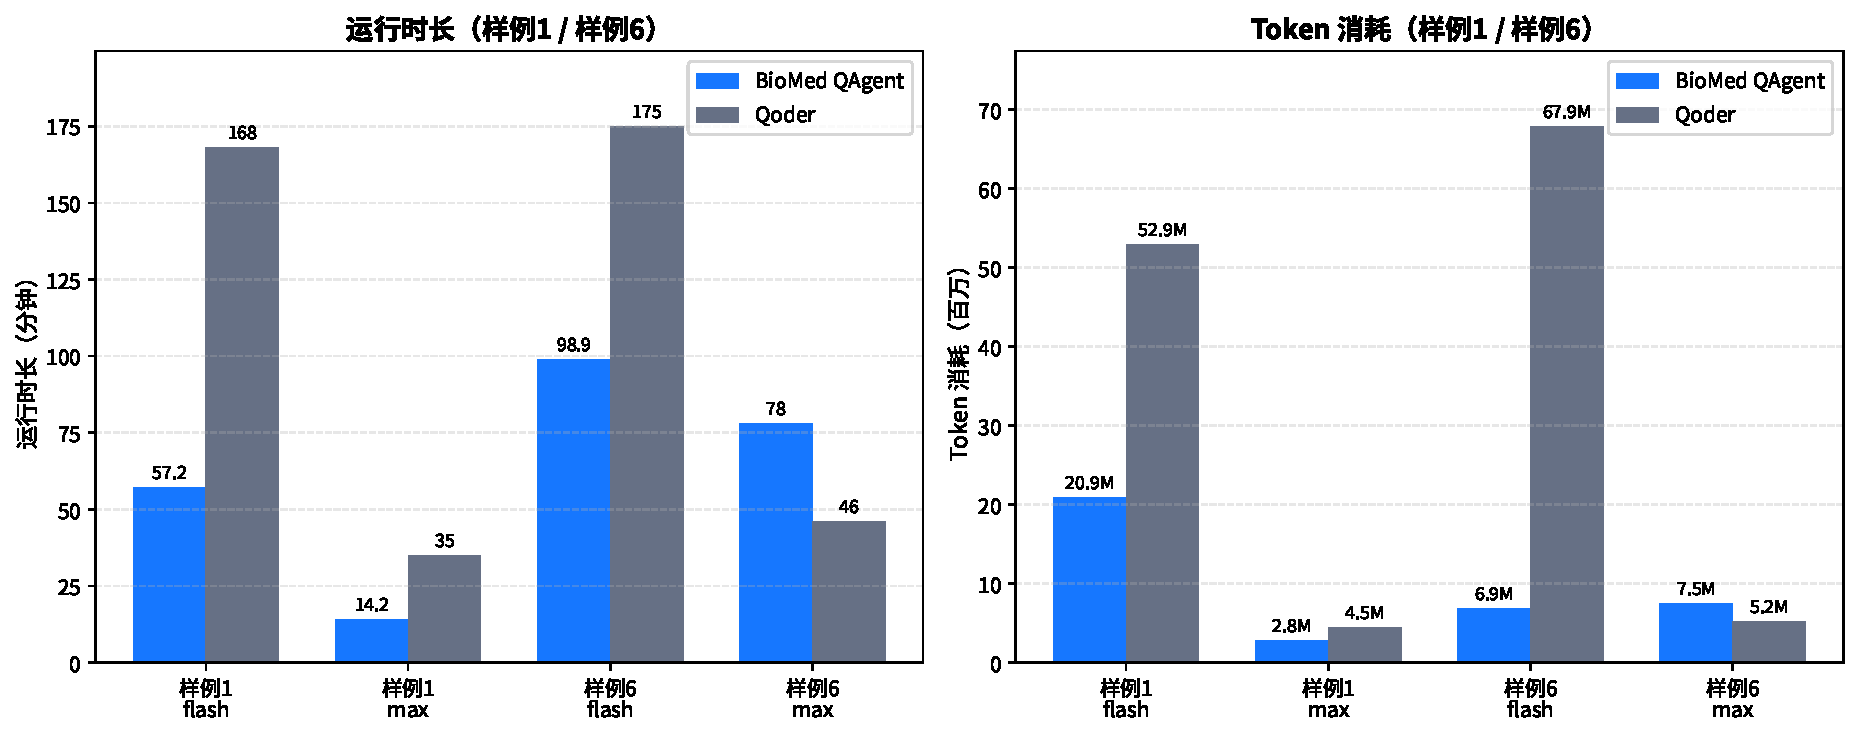
\includegraphics[width=0.97\textwidth]{figures/fig-samples-efficiency-comparison.pdf}
\caption{两案例的运行记录值。来源与计量方式不同，交付内容亦不相同；柱高不能单独用于判断执行效率。}\label{fig:sample-efficiency}
\end{figure}

\subsection{样例1：表达组学数据整合}\label{subsec:gold1-artifact-compare}

需求覆盖按七项任务条目核对：研究纳入、差异表达、样本元数据、平台注释与探针—基因映射、探针水平数据、基因水平数据，以及分析可用性与来源标注。两名评审的记录中，Qoder flash 因探针表仅覆盖16个研究中的5个，该项按部分完成计，总分6.5/7；其余三组为6/7。这个分数不衡量是否查全研究，也不消除纳入研究数的差异。可审计性没有完整四组分项记录，本节仅说明可核对的文件和来源。

\begin{table}[htbp]
\centering
\caption{样例1四组数据产品比较}\label{tab:gold1-artifacts}
\begin{tabularx}{\linewidth}{>{\hsize=0.66000\hsize}L>{\hsize=0.86400\hsize}L>{\hsize=0.90000\hsize}L>{\hsize=1.05600\hsize}L>{\hsize=0.96000\hsize}L>{\hsize=1.56000\hsize}L}
\toprule
\textbf{组} & \textbf{研究数} & \textbf{样本元数据} & \textbf{探针水平} & \textbf{基因水平} & \textbf{证据组织} \\
\midrule
flash · B & 1，GSE86374 & GSM分组支撑表 & 与基因级融合于长表 & 5,294,223行 & 记录级来源定位与发布校验 \\
flash · Q & 16 & 3,226行 & 5个研究宽表 & 13个研究宽表与汇总 & URL、MD5、检索日期、筛选记录 \\
max · B & 2 & GSM分组支撑表 & GSE139038长表 & GSE86374长表 & 记录级来源定位与发布校验 \\
max · Q & 4 & 443行 & 4个研究宽表 & 4个研究宽表 & URL、MD5、质量日志 \\
\bottomrule
\end{tabularx}
\end{table}

交付形态与数据组织。四组产物表现出两种不同的数据组织方式。Qoder 为每个研究输出宽表，每行对应探针或基因、每列对应样本，便于直接进入R 或Python；\mbox{BioMed QAgent} 发布长表，每个样本的每个探针或基因各占一行，并保存记录级来源定位，适合逐行核验和跨来源复用。Qoder flash 纳入16 个研究，\mbox{BioMed QAgent} flash 发布1 个研究，max 发布2 个研究；只有Qoder flash 进一步交付了单研究差异分析和跨研究元分析。

来源定位与质量记录方面，本系统将发布清单与记录定位相连，抽样记录可以定位到原始压缩文件中的具体行；字段类型、单位、映射和溯源检查在发布前执行。样例1 flash 的 GPL6244 探针中，33.3\%没有基因注释，系统保留并标注这些未映射记录。两环境共有记录互查时出现4.1862与4.186等差异，与保留小数位不同相符；由于未核对原始来源，不能据此判定哪一份更准确或证明本系统保留了全部原始精度。

本系统两档均未执行差异表达，纳入研究数也少于 Qoder；记录级溯源还带来存储开销，例如 GSE86374 的规范化日志约0.6 GB。Qoder 以研究宽表及分析结果提供另一种交付形式。本案例呈现了研究范围、表结构、来源粒度和存储成本的取舍，不能仅据总时长认定效率优劣。

运行稳定性。在Qoder flash 运行中，系统发生两次异常中断，由人类手动恢复后继续运行。

\subsection{样例6：文献活性与图表证据}\label{subsec:gold6-artifact-compare}

本案例比较论文与实验记录、补充材料、图表数据，以及来源与置信度说明。由于四组任务条目和证据分项评分尚未全部完成，本节不补填统一覆盖分，而是保留交付结构与离线核对结果。六张表或九件文件只说明发布包的组成，不说明每张表均含有效记录，也不代表已经完成图表曲线数字化。

两份 Qoder 离线包另有结构复用分 X 与证据检查分 Y。X 按模式分解、标识符归一、单位归一、维表、清单和拒绝记录六项取均值；Y 使用来源、定位、清单、方法、检查与原始材料六项。表~\ref{tab:gold6-qoder-2x2}、表~\ref{tab:gold6-qoder-subscores}列出离线评分及其依据。小数分项属于复核者给分，不是数值正确率，也不替代缺少的四组需求评分。

\begin{table}[htbp]
\centering
\caption{样例6两份Qoder离线包的补充评分}\label{tab:gold6-qoder-2x2}
\begin{tabularx}{\linewidth}{>{\hsize=0.55000\hsize}L>{\hsize=0.45000\hsize}L>{\hsize=0.45000\hsize}L>{\hsize=2.55000\hsize}L}
\toprule
\textbf{模型} & \textbf{X} & \textbf{Y} & \textbf{可核对差异} \\
\midrule
flash & 0.950 & 0.808 & 22个CSV；10,682条事实对应10,215个来源位置 \\
max & 0.500 & 0.758 & 结构较紧凑；6,439条事实对应11个来源位置 \\
\bottomrule
\end{tabularx}
\end{table}

\begin{table}[htbp]
\centering
\caption{样例6 Qoder离线包的分项评分}\label{tab:gold6-qoder-subscores}
\begin{tabularx}{\linewidth}{>{\hsize=1.72340\hsize}L>{\hsize=0.63830\hsize}L>{\hsize=0.63830\hsize}L>{\hsize=1.72340\hsize}L>{\hsize=0.63830\hsize}L>{\hsize=0.63830\hsize}L}
\toprule
\textbf{X分项} & \textbf{flash} & \textbf{max} & \textbf{Y分项} & \textbf{flash} & \textbf{max} \\
\midrule
模式分解 & 1.00 & 0.30 & 溯源非空率 & 1.00 & 1.00 \\
标识符归一 & 1.00 & 0.50 & 溯源粒度 & 1.00 & 0.65 \\
单位与剂量归一 & 1.00 & 0.90 & 清单哈希可验证 & 0.60 & 1.00 \\
可复用维表 & 1.00 & 0.10 & 质量检查可复算 & 0.85 & 0.80 \\
清单完整性 & 0.70 & 1.00 & 方法日志深度 & 1.00 & 0.70 \\
拒绝与排除记录 & 1.00 & 0.20 & 原始证据留存 & 0.40 & 0.40 \\
均值 & 0.950 & 0.500 & 均值 & 0.808 & 0.758 \\
\bottomrule
\end{tabularx}
\end{table}

上述分数只描述两份离线包，不能将 X 的0.500视为任务需求覆盖分。表~\ref{tab:gold6-artifacts}进一步列出四组文件结构与可复核内容。

\begin{table}[htbp]
\centering
\caption{样例6四组数据产品的结构与证据}\label{tab:gold6-artifacts}
\begin{tabularx}{\linewidth}{>{\hsize=0.55000\hsize}L>{\hsize=1.15000\hsize}L>{\hsize=1.15000\hsize}L>{\hsize=1.15000\hsize}L}
\toprule
\textbf{组} & \textbf{数据结构} & \textbf{证据与检查} & \textbf{交付内容} \\
\midrule
flash · B & 活性值、实验、论文、补充材料与图表等六个关联表 & 记录级来源与文件摘要 & 当前正式版本共九件文件 \\
flash · Q & 10,682行事实表及筛选、排除、访问记录与维表 & 来源定位较细；清单一处自指摘要不符 & 文件分解较细 \\
max · B & 六个关联表及表结构、溯源和质量评估 & 报告94项检查通过，逐件核验摘要 & 29次模型调用、54次工具调用 \\
max · Q & 6,439行事实表、来源登记与方法日志 & 清单5/5通过；来源定位较粗 & 另含145条GtoPdb策展记录 \\
\bottomrule
\end{tabularx}
\end{table}

交付形态与数据组织。两份Qoder 主表都包含记录编号、突变体、化合物、ChEMBL 标识、活性类型、纳摩尔值、细胞系、来源数据库、检索日期、抽取方法和置信度等核心字段。flash 主表为10,682 $\times$ 109，还提供以摩尔浓度负十进制对数表示的pXC、跨源一致性、化合物身份解析、证据文本以及表格行列坐标；max主表为6,439 $\times$ 35，结构更紧凑，并额外纳入145条GtoPdb（药理学指南数据库）策展记录。flash 还把单剂量筛选、非浓度指标、排除记录、拒绝候选、补充材料访问、未解析附件和参考维表拆为独立文件，这些文件说明它保留了哪些处理结果，不以文件数量代替需求完成程度。

来源定位与质量证据。来源粒度进一步区分了两套产品。flash 的10,682 条事实对应10,215 个不同来源位置，包括ChEMBL 活性标识、表格行列坐标、证据文本和补充材料工作表定位；max 的6,439 条事实只有11 个不同的来源定位值，其中6,285 行共享同一说明。因此，两者来源字段均非空，但flash 更接近记录级定位，max 更接近来源批次级定位。

清单复算方面，Qoder flash 的22个文件在行数、列数和大小上均匹配，21/22个 SHA-1 前缀可验证；清单自指行不匹配，且摘要只保留16位十六进制前缀。其质量检查中，唯一性、正值范围、pXC、一致性分类与来源计数可以复算；部分组合中位数因筛选条件未完整说明，只能复现相对高低。max 的5个清单条目 MD5 全部通过，行列数与来源非空情况也可复算。两份包均缺少方法日志引用的原始响应、附件、图件与提取脚本，无法仅凭离线包重放全过程。

本系统两档将六张关联表及三件说明文件作为当前正式版本交付。flash 先后发布两个版本，第二次明确替代第一次并保留关联；max 记录了94项检查。这样的发布组织便于核对文件、来源和检查结果，但检查数量不代表科学正确率。两环境还存在图表、附件与记录范围差异，本节没有证明同等任务和质量下的效率优势。

\begin{figure}[htbp]
\centering
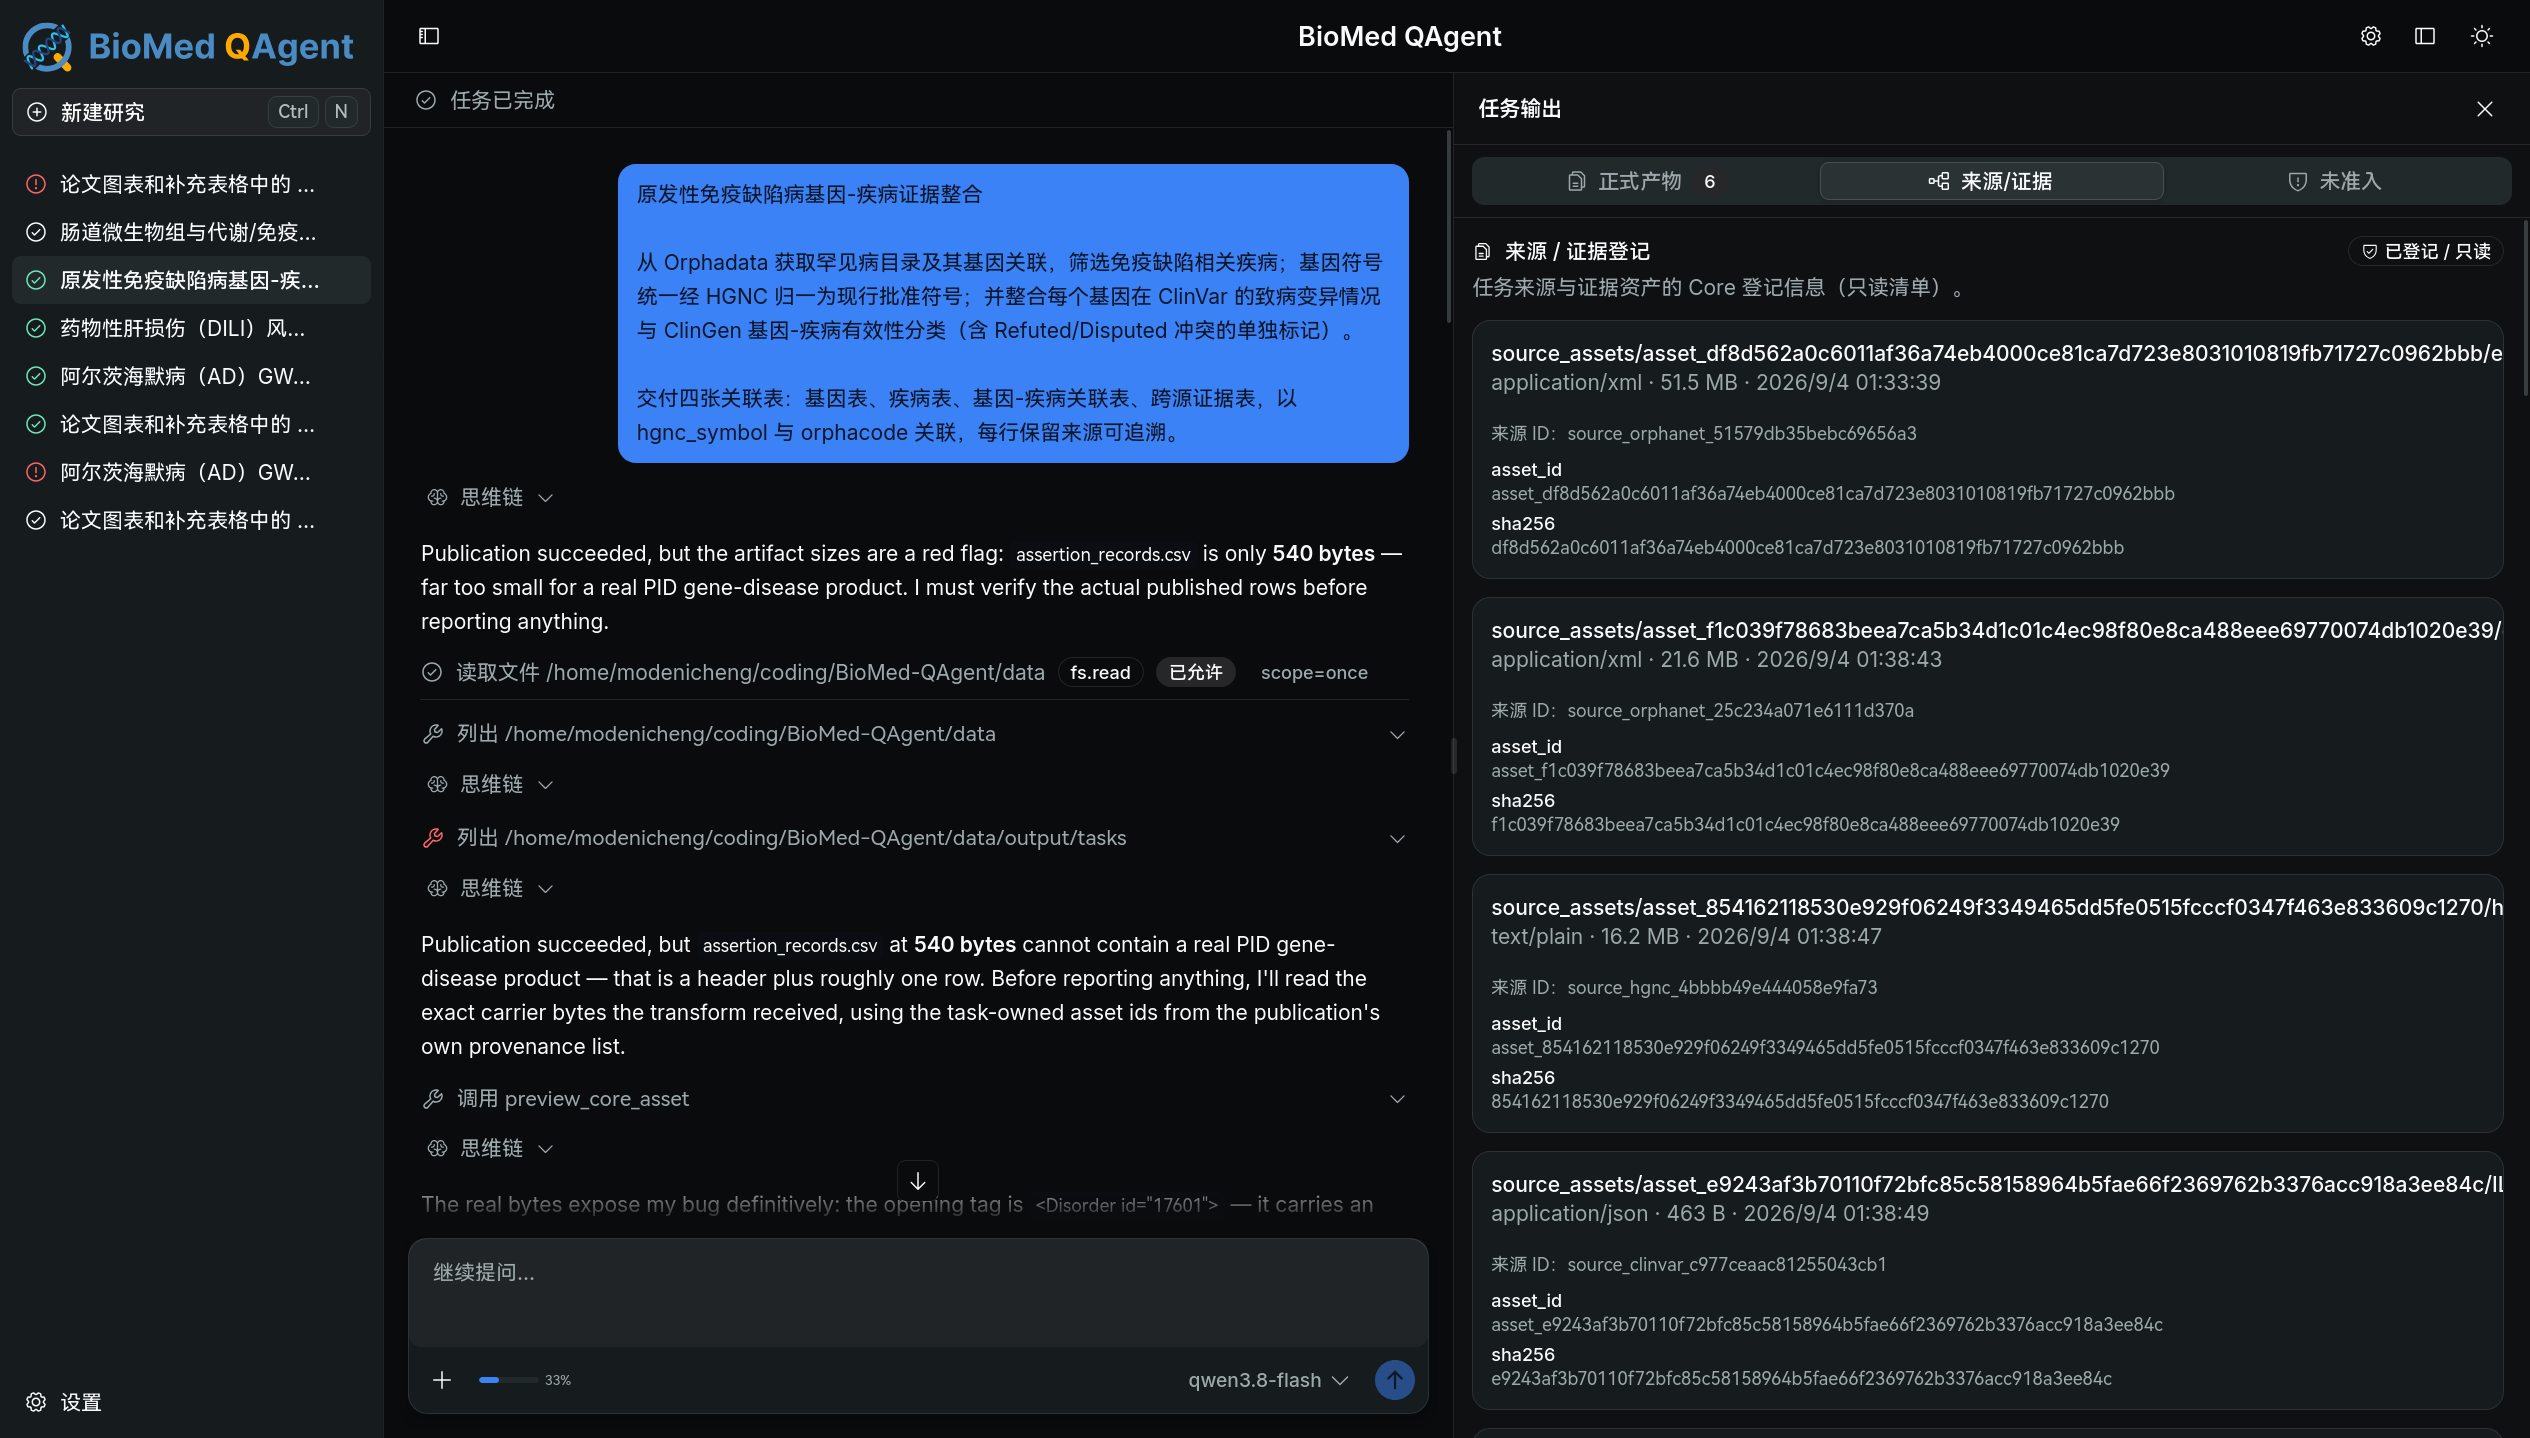
\includegraphics[width=0.93\textwidth]{figures/ui-gold6-table-topology.png}
\caption{样例6正式发布物的表关系与文件组织。}\label{fig:ui-gold6-topology}
\end{figure}

\subsection{主要发现}

首先，本系统将正式发布与可核验文件相连，并在发布前保存字段、关系、来源和质量检查结果。样例1保留未映射探针，样例6组织关联表并保留修改后的发布版本。

其次，文件存在、通过检查和满足原始需求是不同结果。Qoder 的离线包也包含来源与质量记录，不能将它概括为只有聊天回答；本系统的正式发布身份同样不能代替需求覆盖和来源级数值核对。

最后，运行记录显示成本有差异，但交付规模、内容与计量方式尚未统一。较低总量可能同时对应较少交付，不能排除这一解释。本文因此将成本作为观察结果，不据此宣称本系统或某个模型档位更高效。

\section{部署与视频演示}\label{sec:video-demo}

随报告提交的视频演示展示了一次从零开始的独立部署与运行，验证系统不依赖开发环境即可安装和使用：

\begin{enumerate}
  \item 安装与启动：下载正式 release 后运行，无需从源码构建。
  \item 模型配置：在前端设置 qwen3.8-flash 与 API 密钥，界面见图~\ref{fig:ui-settings-models}。
  \item 完全人工审批：演示运行样例7时配置人工审核，流程中出现一次确认，处理后继续并形成正式发布。此演示与表~\ref{tab:gold-overview}的归档运行不是同一次。
  \item 外部来源扩展：配置 ClinicalTrials.gov，查询“2型糖尿病目前有哪些临床试验？给出3个NCT编号、题目和状态”，检查返回字段。该演示只说明这条调用路径，不作为全面检索能力评测。
\end{enumerate}

视频补充了安装、配置、人工处理和继续运行的可见过程。它不补足十二次评测中的全部审批记录，也不证明所有动态发布路径都会自动发起人工验收。

\section{本章小结}

十个案例中，九个至少形成一次正式发布，一个因必需数据缺失而停止；加上两次 max 观察，共十二次运行，十一次正式发布。已交付文件、未完成需求与运行成本分别记录。跨环境比较显示不同系统在研究范围、文件组织和来源定位方面各有差异；当前证据支持描述这些差异，不支持等工作量下的效率排序、科学正确率或查全率结论。


\chapter{总结与讨论}

\section{适用范围与额外开销}

本节从使用流程讨论系统可能减少哪些重复操作、增加哪些开销，不作为人工实验基线。第五章实际比较对象是 Qoder，并未测量纯人工完成任务的时间与成本。

\begin{table}[htbp]
\centering
\caption{不同工作方式与本系统的额外开销}\label{tab:benefit-cost}
\begin{tabularx}{\linewidth}{>{\hsize=0.60000\hsize}L>{\hsize=1.20000\hsize}L>{\hsize=1.20000\hsize}L}
\toprule
\textbf{工作方式} & \textbf{本系统希望减少的重复操作} & \textbf{仍需承担的开销} \\
\midrule
人工整理 & 多库查询、重复下载、复制对列、检查重复与冲突，以及补写来源说明 & 模型调用、文件存储、摘要计算、来源适配及人工复核 \\
依靠对话与临时脚本 & 寻找当前文件、补记处理步骤、追查来源及确认哪些结果可以交付 & 维护表结构与解析器、执行检查、保存过程记录和发布版本 \\
\bottomrule
\end{tabularx}
\end{table}

系统并不消除人工，而是让研究者少做重复整理，将注意力放在来源选择、字段含义、冲突与不确定记录上。能减少多少人工工作，仍需另行测量。

\section{对科研数据适用性的实际意义}

发布包将数据表、来源、检查结果与版本记录一并保存。研究者可以按明确的连接键使用多表数据，也能在发现问题时回查并修正。它减少了交付文件缺少说明、不同成员持有不同版本的风险，但是否适合某项分析，仍需结合研究任务判断。

\section{实验结果的关键发现}\label{sec:findings-validation}

十二次列示运行中，十一次正式发布，一次未发布，汇总比例为91.7\%。样例10缺少必需输入，因而没有正式交付。发布状态与需求完成情况必须分别记录；这个比例不代表原始需求全部满足，也不是统一条件下的成功概率。

两案例的 flash 记录成本均是本系统较低，样例6 max 则是 Qoder 较低。交付范围与计量方式不同，无法据此区分执行效率、工作量与其他运行条件的影响。

本系统保存发布清单、来源与检查结果；Qoder 样例6两份离线包也有来源列、清单和方法日志，但缺少所引用的原始文件与脚本。两者便于复核的程度不同，不等于已经测得数值正确率。

\section{核心机制的实际表现}

\textbf{正式发布与文件核验。}成功运行具有可检查文件，未发布运行保留原因。摘要重验确认了既有文件与回执一致，未检验冻结输入后的跨次重跑。

\textbf{运行时表结构检查。}样例7、9展示了动态路线的执行与发布。样例9采用的产品不同于原静态四表规格，不能视作同范围任务已经全部完成；新领域适用范围与变换计算仍需另行检验。

\textbf{证据绑定的人工确认。}样例6 flash 记录三次来源访问授权、两次发布验收及两个版本的替代关系。该记录说明相应步骤实际执行过，但不足以评估模型初审准确率；零 HIL 的动态案例也不证明所有路径均强制触发人工验收。

\section{结论}

\mbox{BioMed QAgent} 将研究需求依次转换为检索、采集、解析、整合与正式交付。Agent 提出查询、来源、多表规格和修改建议，Dataset Core 检查候选并控制正式写入，文件与处理记录随版本保存。

本轮运行展示了可核验交付、缺少必要数据时拒绝发布，以及保留修改历史三项行为。后续应优先核对原始字段与数值、检查明确范围内的参考来源，并在冻结输入、代码和参数后重跑。系统旨在让数据交付有据可查，不以发布成功替代科学判断。

\renewcommand{\bibname}{参考文献}
\begin{thebibliography}{9}
\bibitem{langgraph} LangChain. LangGraph: Interrupts [EB/OL]. \url{https://docs.langchain.com/oss/python/langgraph/interrupts}. 2026-09-06查阅。
\bibitem{autogen} Wu Q., Bansal G., Zhang J., et al. AutoGen: Enabling Next-Gen LLM Applications via Multi-Agent Conversation [EB/OL]. arXiv:2308.08155, 2023.
\bibitem{openai-agents} OpenAI. OpenAI Agents SDK [EB/OL]. \url{https://openai.github.io/openai-agents-python/}. 2026-09-06查阅。
\bibitem{docetl} Shankar S., Parameswaran A. G., Wu E. DocETL: Agentic Query Rewriting and Evaluation for Complex Document Processing [EB/OL]. arXiv:2410.12189v1, 2024.
\bibitem{palimpzest} Liu C., Russo M., Cafarella M., et al. A Declarative System for Optimizing AI Workloads [EB/OL]. arXiv:2405.14696v2, 2024.
\bibitem{temporal-approval} Temporal Technologies. Workflow message passing [EB/OL]. \url{https://docs.temporal.io/encyclopedia/workflow-message-passing}. 2026-09-06查阅。
\bibitem{qoder} Qoder. 什么是Qoder [EB/OL]. \url{https://docs.qoder.com/zh/product-series/what-is-qoder}. 2026-09-06查阅。
\bibitem{biomed-evidence} BioMed-QAgent项目组. Gold6–10 Corrected Campaign Session Report [EB/OL]. 实验代码版本：e5aadfe0；归档目录：\path{docs/evaluation/gold6-10-2026-09-03/}，2026。
\end{thebibliography}



% ------------------------- 附录 -------------------------
\appendix

% 章标题编号呈“附录 A”格式（见 theme 中 ReportChapterLabelPrefix）
\renewcommand{\ReportChapterLabelPrefix}{附录~}

% =====================================================================
% 附录 A — 网盘文件说明
%
% 网盘随附文件清册。
% 列宽策略:文件名列定宽(\seqsplit 断词 + \texttt),说明列吃掉
% 全部剩余宽度;避免长文件名把说明列挤到重叠。
% =====================================================================

\chapter{网盘文件说明}\label{app:cloud-files}

为控制正文篇幅，部分大体积文件（安装包、系统架构图、演示视频等）不随正文装订，以网盘形式随作品提交。表~\ref{tab:cloud-files}列出网盘目录下的全部文件及其内容说明，供评审对照查阅。

\begin{table}[htbp]
\centering
\caption{网盘文件清单}\label{tab:cloud-files}
\begin{tabularx}{\linewidth}{@{}>{\raggedleft\arraybackslash}p{2.4em} l >{\raggedright\arraybackslash}X@{}}
\toprule
\textbf{序号} & \textbf{文件名} & \textbf{内容说明} \\
\midrule
1 & \seqsplit{BioMed-QAgent-1.0.0-win.zip} & Windows 安装包。 \\
2 & \seqsplit{BioMed-QAgent-1.0.0-x86\_64-Linux.AppImage} & Linux x86\_64 安装包。 \\
3 & \seqsplit{BioMed-QAgent-1.0.0.zip} & 纯构建产物，不包含运行环境。使用前需自行安装并配置 Python、uv 和 pnpm。 \\
4 & \seqsplit{biomed-qagent-main.pdf} & 系统架构图。 \\
5 & \seqsplit{qwen调用凭证.png} & Qwen 调用凭证。 \\
6 & \seqsplit{video.mp4} & 系统演示视频。 \\
\bottomrule
\end{tabularx}
\end{table}


\end{document}
